%\documentclass[table, 10pt]{beamer}%
\documentclass[table, 10 pt, handout]{beamer}%

\usepackage[french]{babel}
\usepackage{tikz}
\usepackage[latin1]{inputenc}
\usepackage{times}
\usepackage[T1]{fontenc}

\usepackage{graphicx,graphics}

\usepackage{amsmath,amsfonts}

\usepackage{multirow}

%\usepackage[table]{xcolor}

%\usepackage{beamerthemeliris}

\usepackage{beamerthemesplit}
\usetheme{Malmoe}%Copenhagen%Dresden%Malmoe
\usecolortheme{orchid}%beetle,seagull,crane,dove,orchid
\useinnertheme[shadow]{rounded}%rounded
\usefonttheme{professionalfonts}

\definecolor{darkgreen}{RGB}{0,180,0} 

\setbeamertemplate{navigation symbols}{}


\newenvironment{codeblock}[1]{\begin{exampleblock}<+->{\texttt{#1}}\begin{tt}}{\end{tt}\end{exampleblock}}




\title[S21 - Comprendre les r�seaux -- CM - Communication par socket, \hspace{1cm}\insertframenumber{} / \inserttotalframenumber]
{S21 -- Comprendre les r�seaux }
\subtitle{CM -- Communication par socket}
\author[Julien Gossa]{Julien Gossa}
\institute
{ 
	{\bf IUT Robert Schuman -- D�partement Informatique}\\
	{\url{julien.gossa@unistra.fr}}
}

\date{2009}
\beamertemplatetransparentcovereddynamicmedium 

\begin{document}


\begin{frame}
 	\titlepage
\end{frame}



\AtBeginSection[]
{
   \begin{frame}
       \frametitle{Sans transition\ldots}
       %\small
       \tableofcontents[currentsubsection]
   \end{frame}
}	

\AtBeginSubsection[]
{
   \begin{frame}
       \frametitle{Sans transition\ldots}
       %\small
       \tableofcontents[currentsubsection]
   \end{frame}
}	

%----------------------------------------------------------------------
\begin{frame}

	\begin{block}<+->{Architectures applicative}
		\begin{itemize}
		\item Gestion des communications au sein d'une application
		\item Choix :
			\begin{itemize}
			\item Quoi �changer ? (Donn�es totales ou mises � jour)
			\item Comment �changer ? (protocole)
			\end{itemize}
		\item D�pend de :
			\begin{itemize}
			\item Objectifs (Nature de l'application)
			\item Donn�es (Taille, Fr�quence des mise � jour)
			\item Contraintes (Performance, Fiabilit�)
			\end{itemize}
		\item En g�n�ral 
			\begin{itemize}
			\item plus de performance = moins de fiabilit� 
			\item et vice versa
			\end{itemize}		
		\end{itemize}		
	\end{block}
	
	\begin{alertblock}<+->{Deux modes de communications principaux}
		\begin{itemize}
		\item D�connect� (UDP) et Connect� (TCP)
		\end{itemize}		
	\end{alertblock}	
\end{frame}
% ----------------------------------------------------------------------


%----------------------------------------------------------------------
\section{Notion de port}
% ----------------------------------------------------------------------
\subsection{Plusieurs applications}
% ----------------------------------------------------------------------
\begin{frame}{Liaison physique}
	
	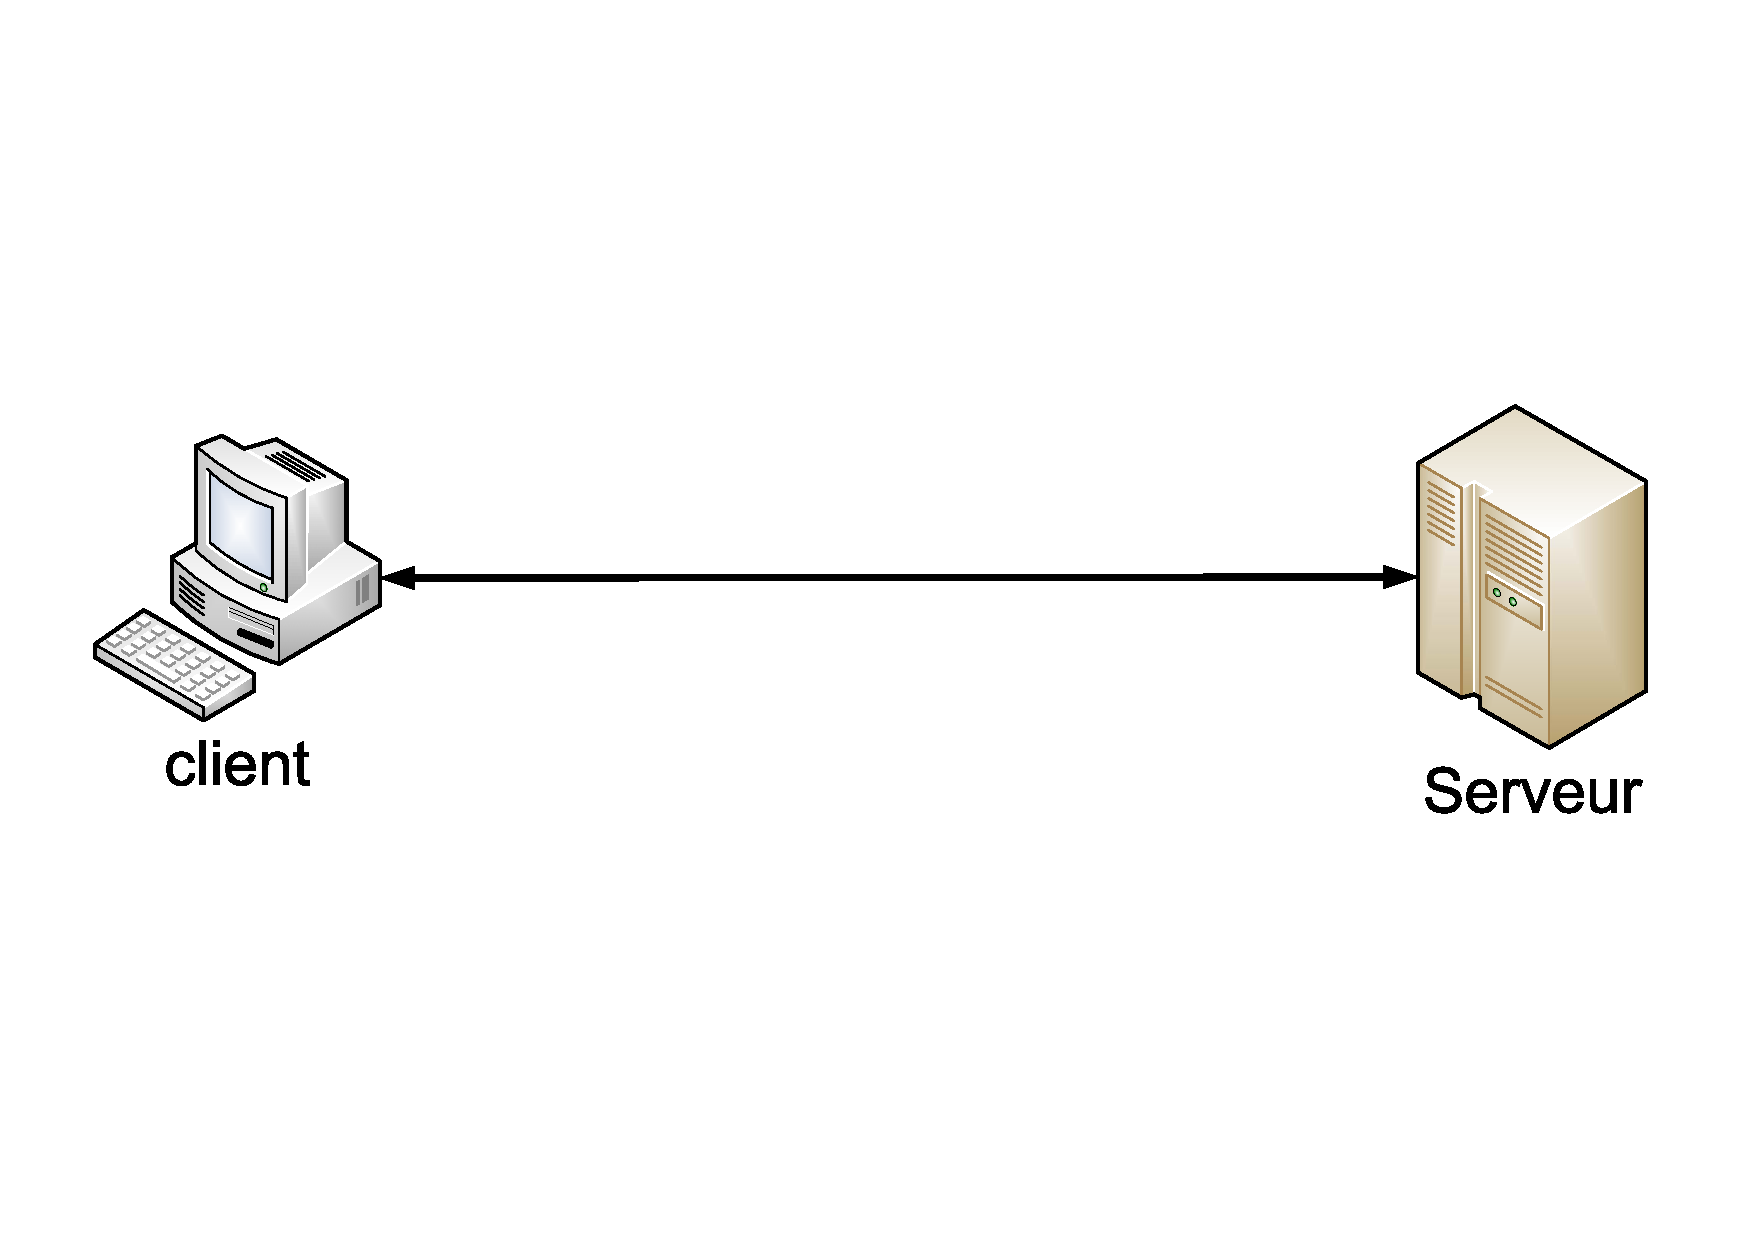
\includegraphics[width=\textwidth]{res/CS1.pdf}
		
\end{frame}
% ----------------------------------------------------------------------
\begin{frame}{Liaison physique : plusieurs applications}

	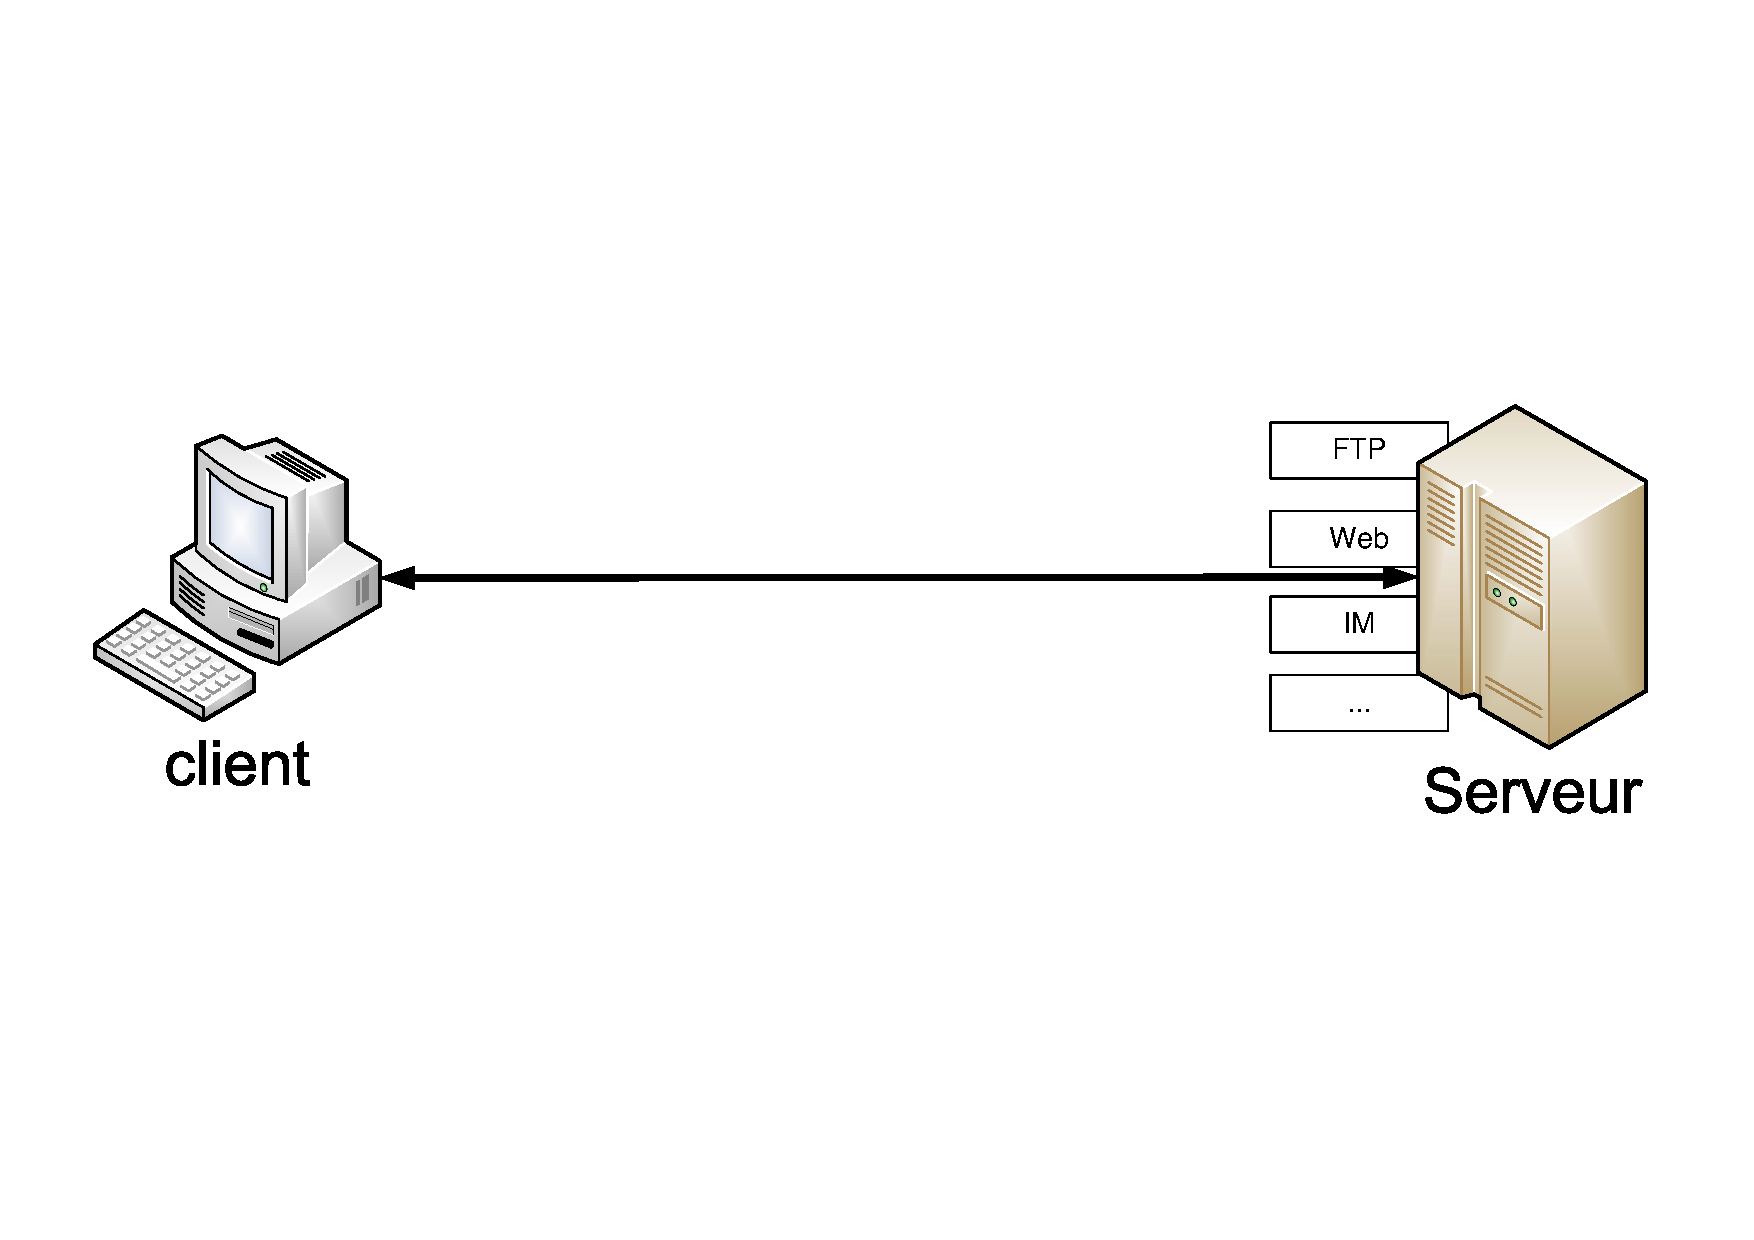
\includegraphics[width=\textwidth]{res/CS2.pdf}
		
\end{frame}
% ----------------------------------------------------------------------
\begin{frame}{Liaison logique : plusieurs cannaux de communication}
	
	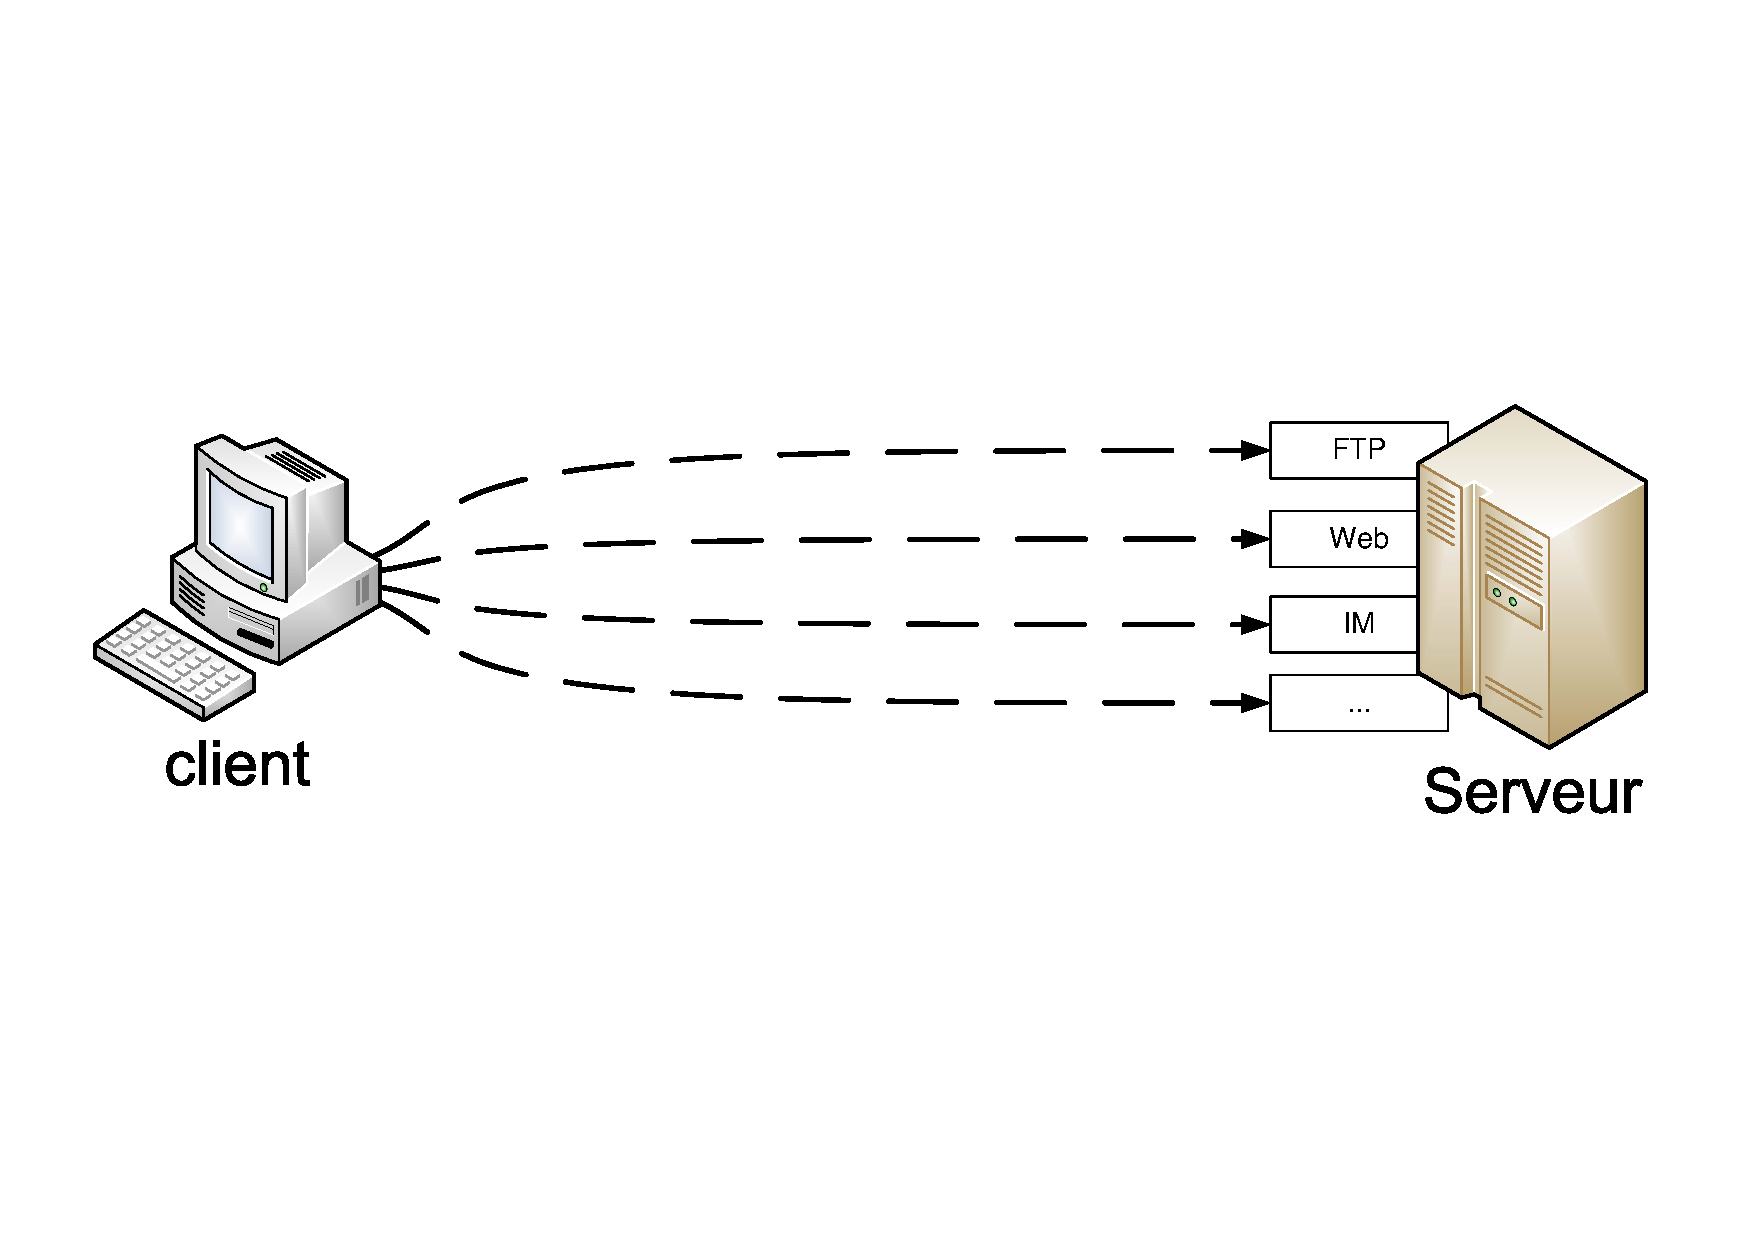
\includegraphics[width=\textwidth]{res/CS3.pdf}
		
\end{frame}
% ----------------------------------------------------------------------
\begin{frame}{Liaison logique : s�paration par \textit{port}}

	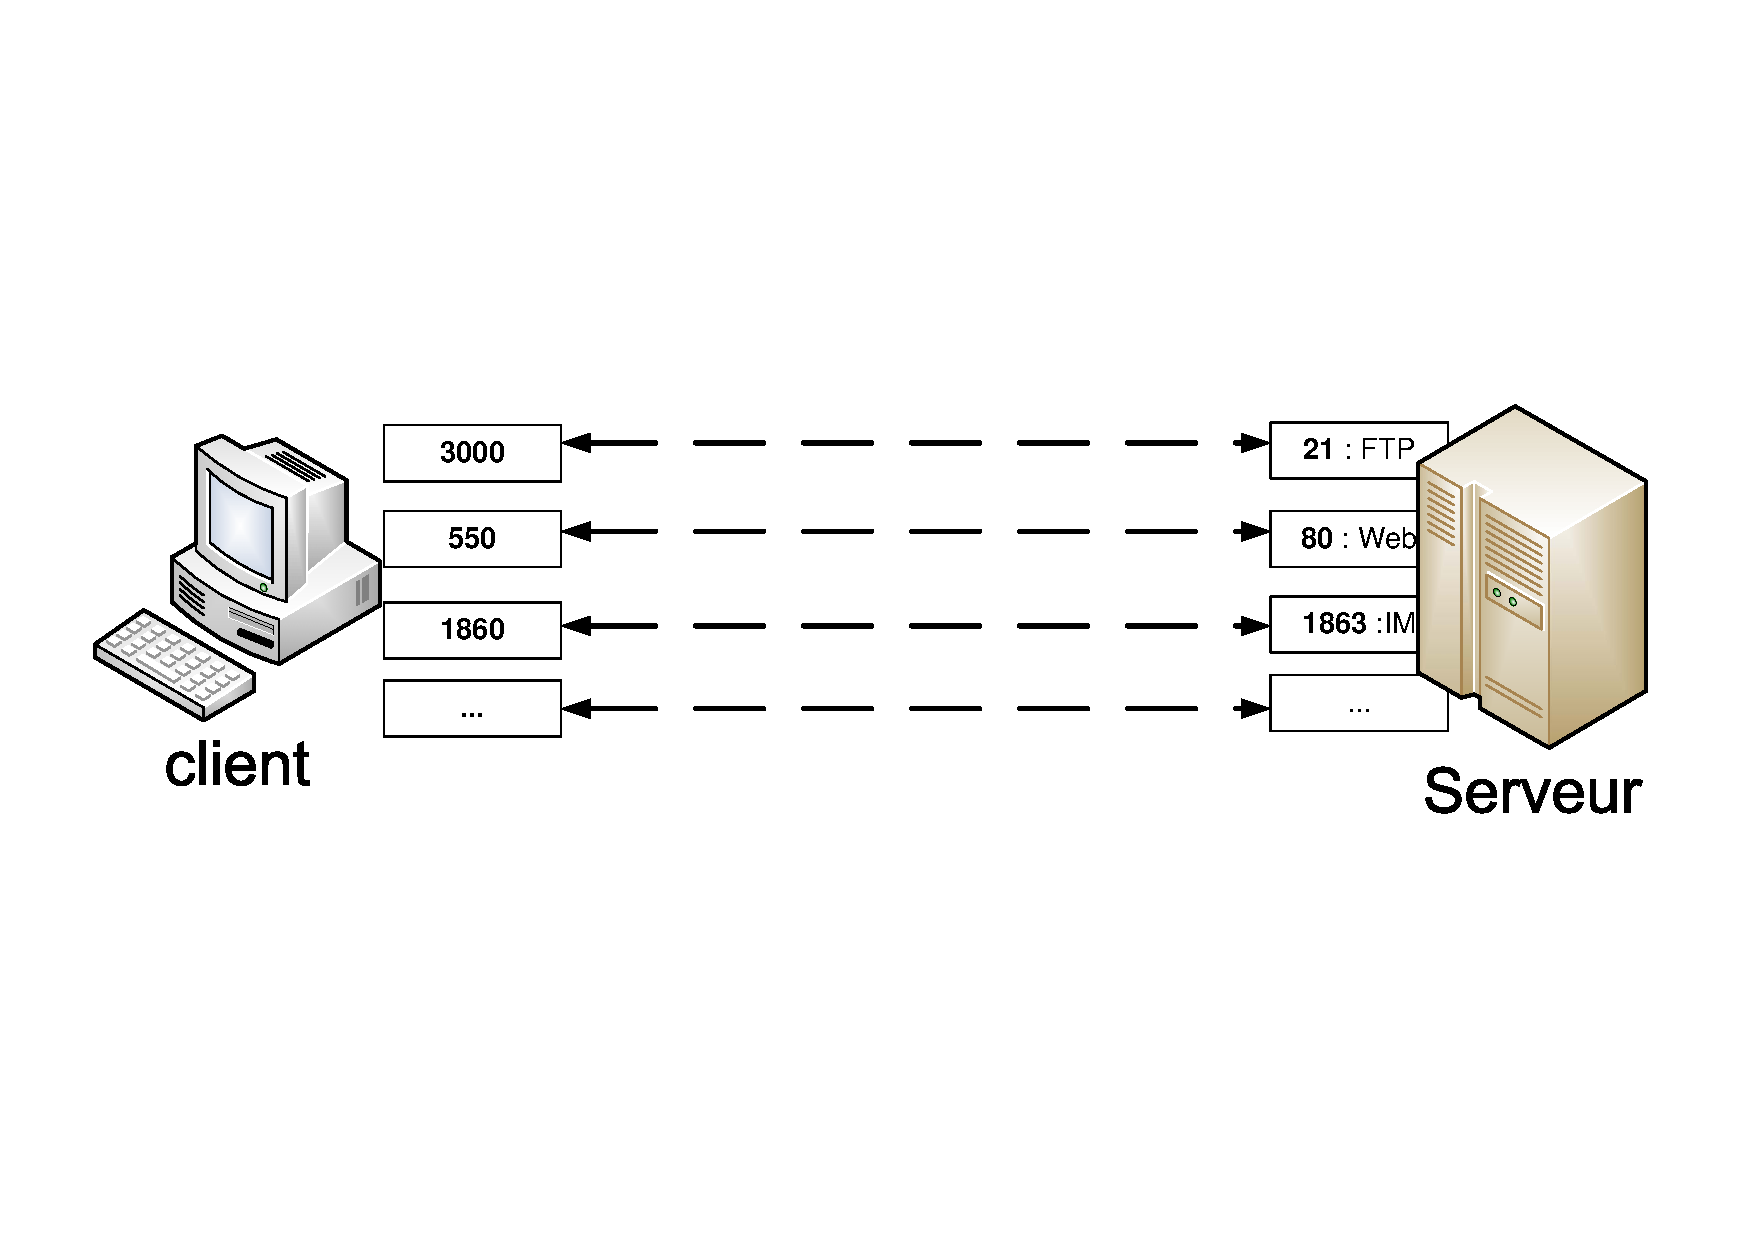
\includegraphics[width=\textwidth]{res/CS4.pdf}
		
\end{frame}
% ----------------------------------------------------------------------

% ----------------------------------------------------------------------
\begin{frame}

	\begin{block}<+->{Notion de port}
		\begin{itemize}
		\item Nombre sur 16 bits (0 � 65535)
		\item Permet de multiplexer les liaisons applicatives dans une liaison physique
		\item Trois cat�gories :
			\begin{itemize}
			\item[0-1023] : ports connus (\textit{Well Known Ports}) 
			\item[1024-49151] : ports enregistr�s (\textit{Registered Ports}) 
			\item[49152-65535] : Ports dynamiques et/ou priv�s (\textit{Dynamic and/or Private Ports}) 
			\end{itemize}
		\item G�r�s par l'IANA (Internet Assigned Numbers Authority)
			\begin{itemize}
			\item \url{http://www.iana.org/assignments/port-numbers}
			\end{itemize}
		\end{itemize}		
	\end{block}
	
	\begin{alertblock}<+->{Exemple}
		\begin{itemize}
		\item Protocole FTP
		\item Construit au dessus de TCP
		\end{itemize}		
	\end{alertblock}	
\end{frame}
% ----------------------------------------------------------------------

% ----------------------------------------------------------------------
\subsection{Plusieurs cannaux de communication}
% ----------------------------------------------------------------------
\begin{frame}{FTP : connexion au port 21}

	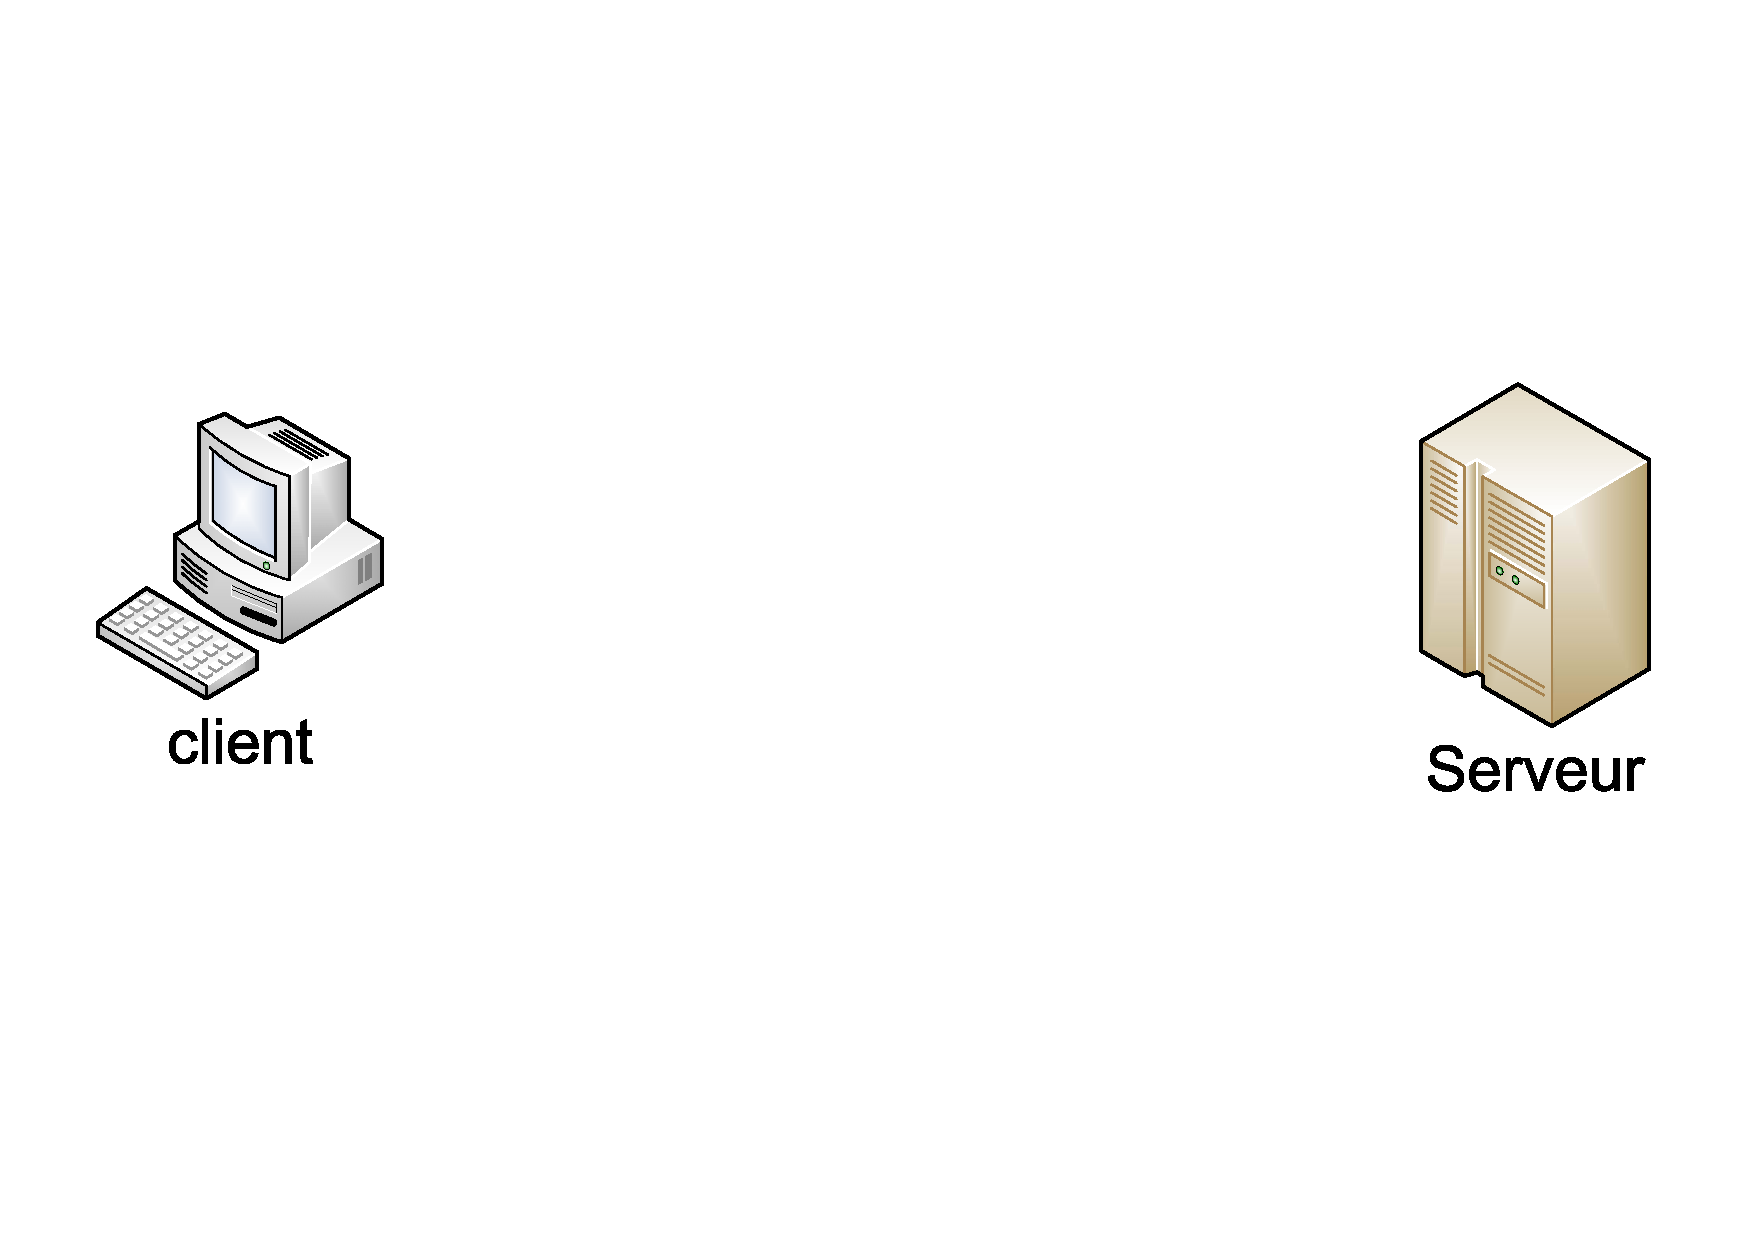
\includegraphics[width=\textwidth]{res/CSftp1.pdf}
		
\end{frame}
% ----------------------------------------------------------------------
\begin{frame}{FTP : plusieurs ports par application}

	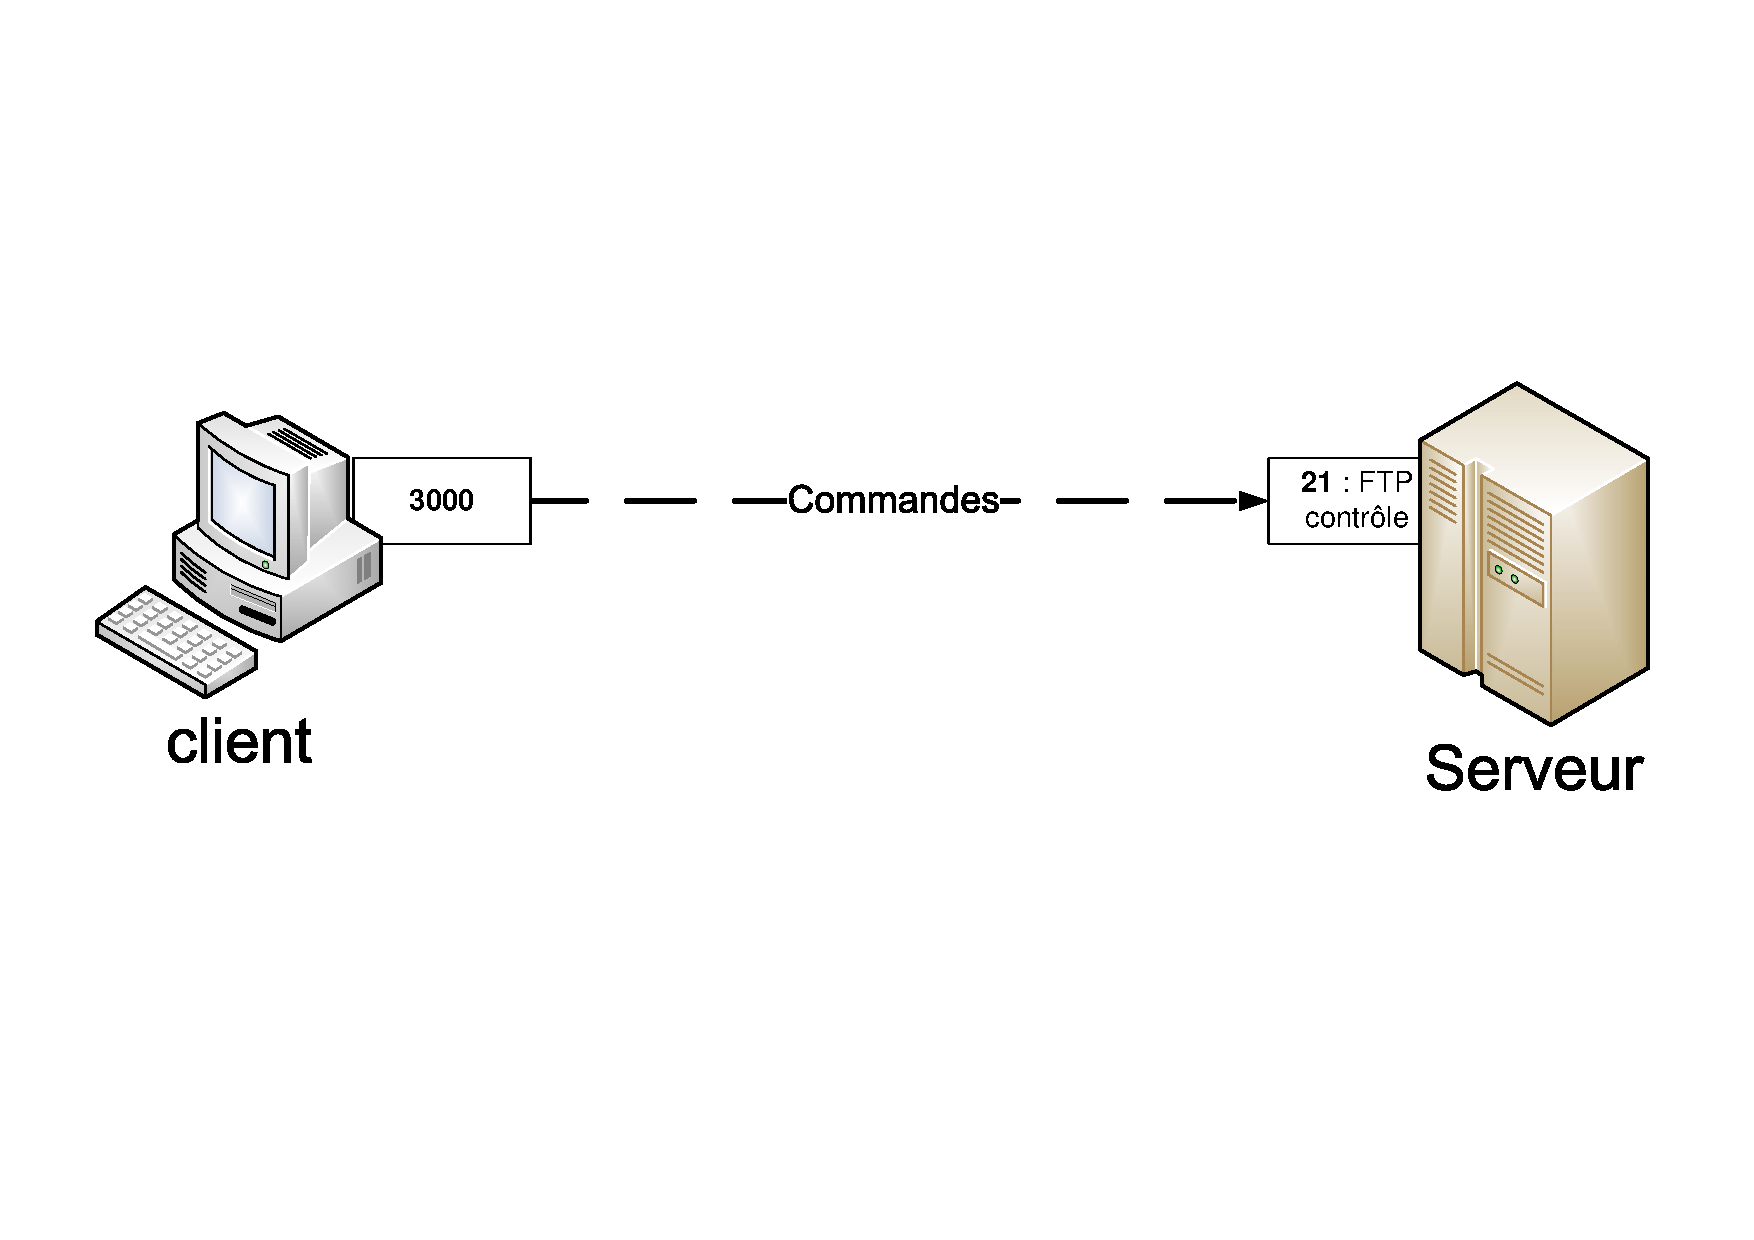
\includegraphics[width=\textwidth]{res/CSftp2.pdf}
		
\end{frame}
% ----------------------------------------------------------------------
\begin{frame}{FTP : fichier suppl�mentaire}

	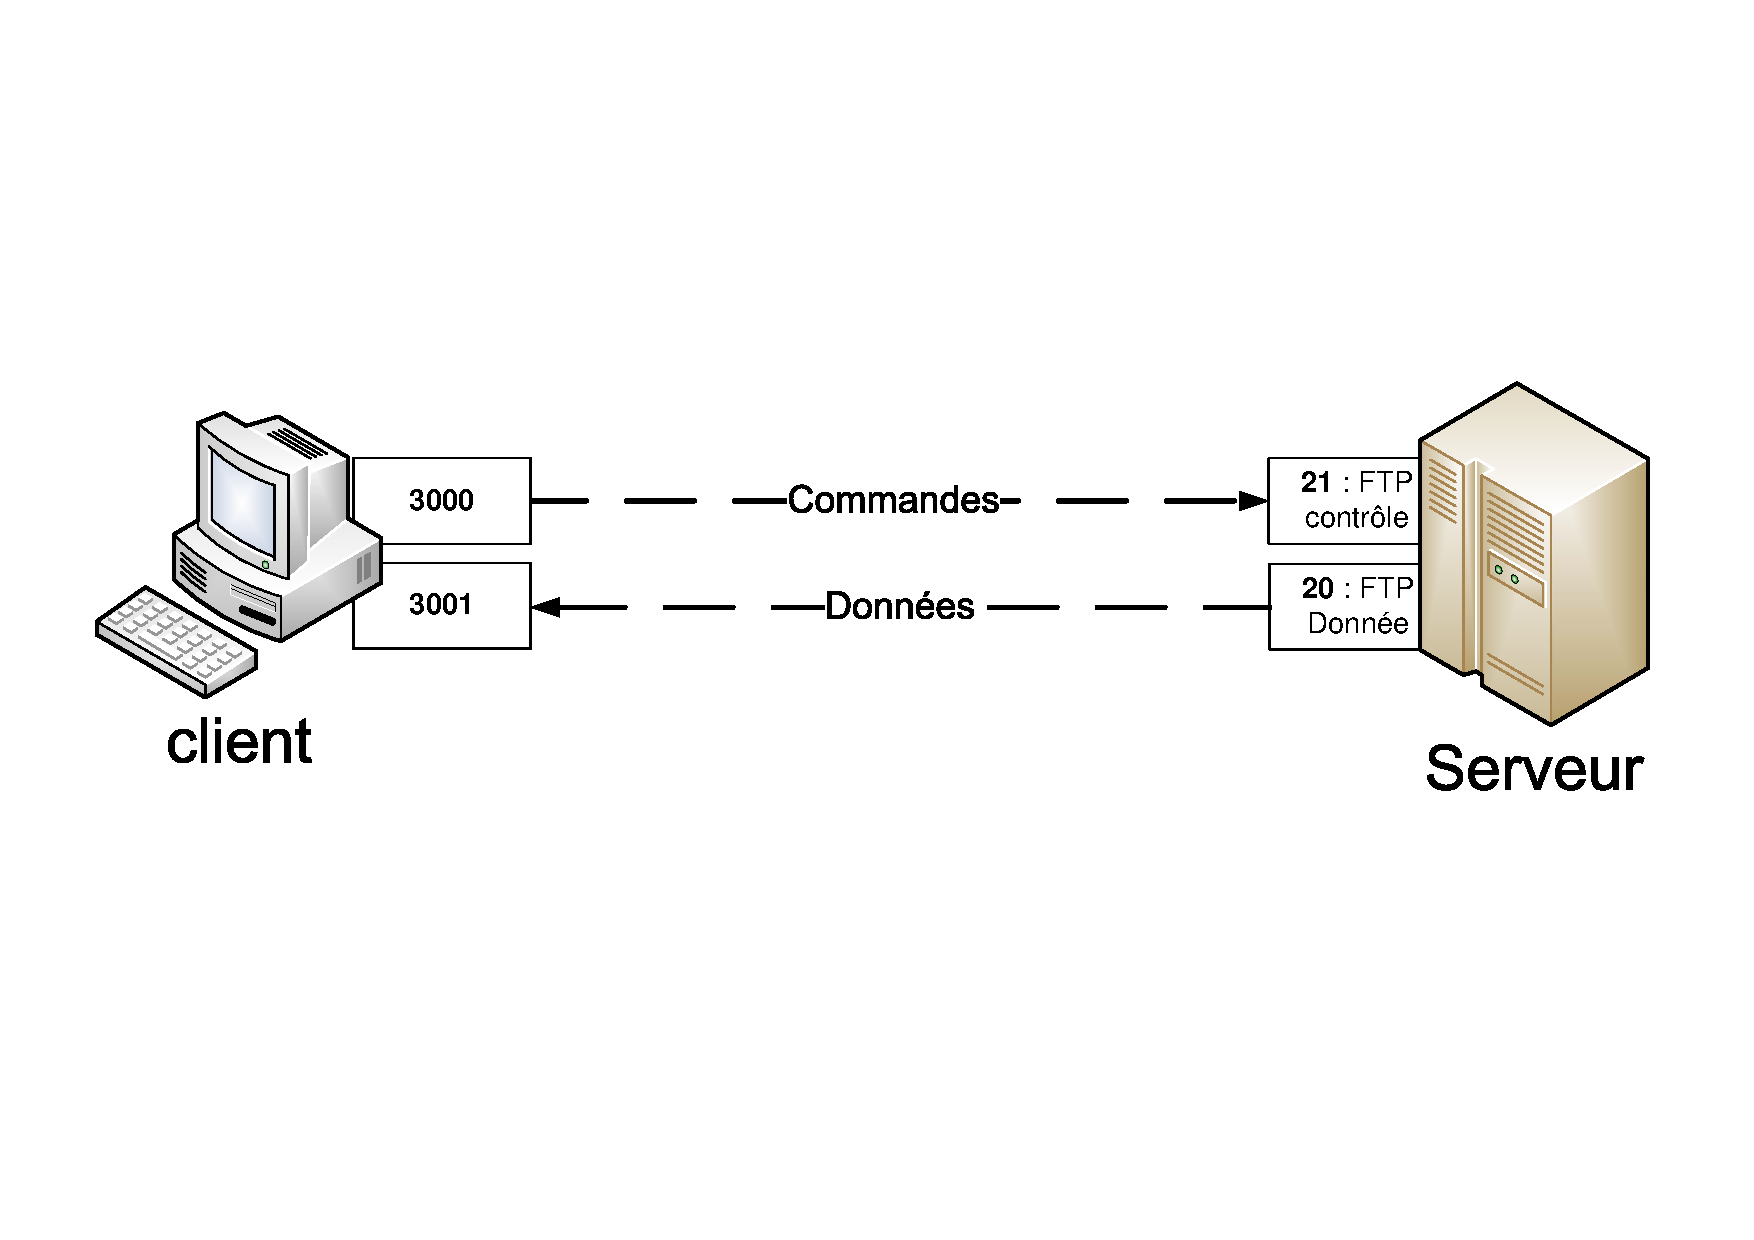
\includegraphics[width=\textwidth]{res/CSftp3.pdf}
		
\end{frame}
% ----------------------------------------------------------------------
\begin{frame}{FTP : encore un fichier suppl�mentaire}

	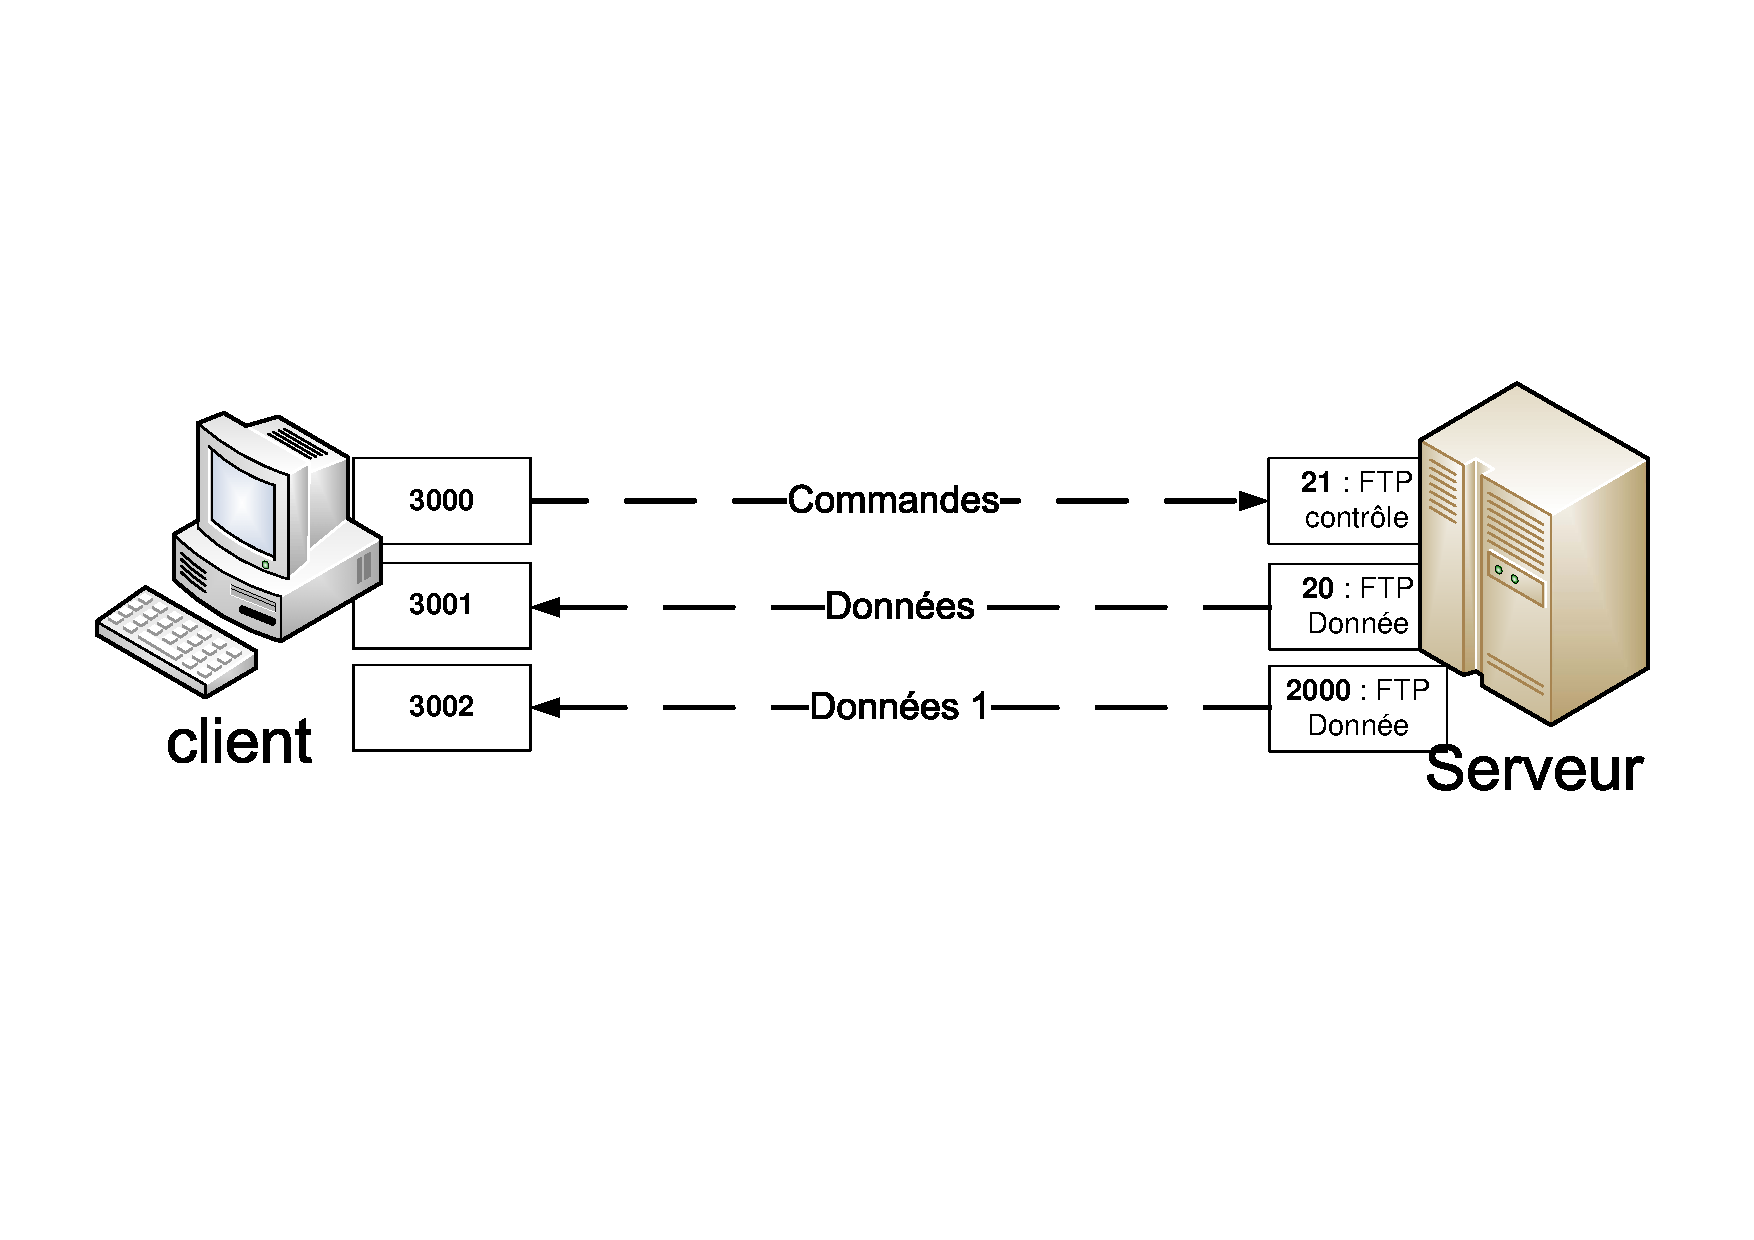
\includegraphics[width=\textwidth]{res/CSftp4.pdf}
		
\end{frame}
% ----------------------------------------------------------------------
\begin{frame}{FTP : encore un fichier suppl�mentaire}

	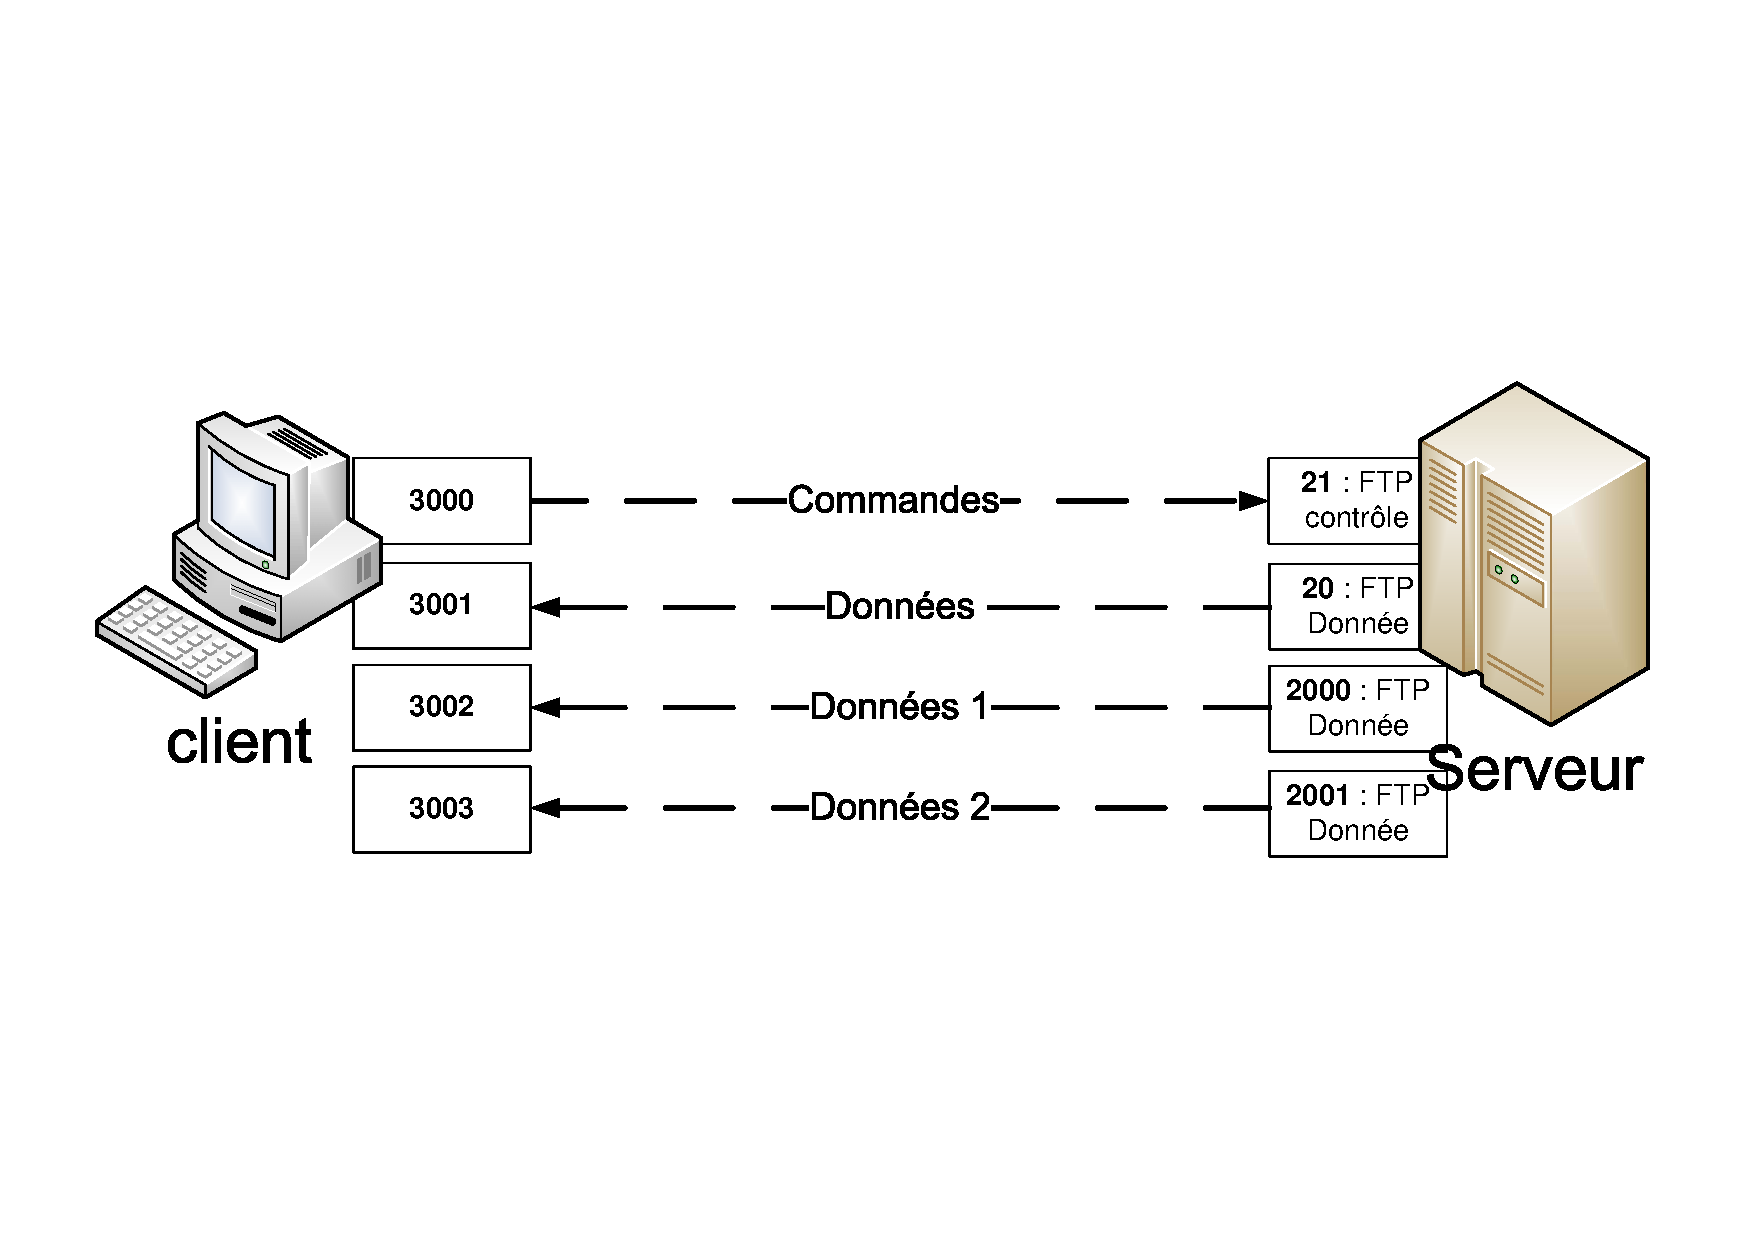
\includegraphics[width=\textwidth]{res/CSftp5.pdf}
		
\end{frame}
% ----------------------------------------------------------------------


% ----------------------------------------------------------------------
\section{Session UDP}
% ----------------------------------------------------------------------
\begin{frame}
	\begin{block}<+->{Protocole UDP}
		\begin{itemize}
		\item \textit{User Datagram Protocol}
		\item Construit par dessus IP
		\item D�fini par la RFC768 
			\begin{itemize}
			\item \url{http://tools.ietf.org/html/rfc768}
			\end{itemize}
		\item Int�gre la notion de port
		\item En mode d�connect�
			\begin{itemize}
			\item performant (peu de surcharge)
			\item peu fiable (perte, int�grit� et ordonnancement des paquets)
			\end{itemize}
		\end{itemize}
	\end{block}
\end{frame}
% ----------------------------------------------------------------------
\begin{frame}{UDP : client/serveur en mode d�connect�}

	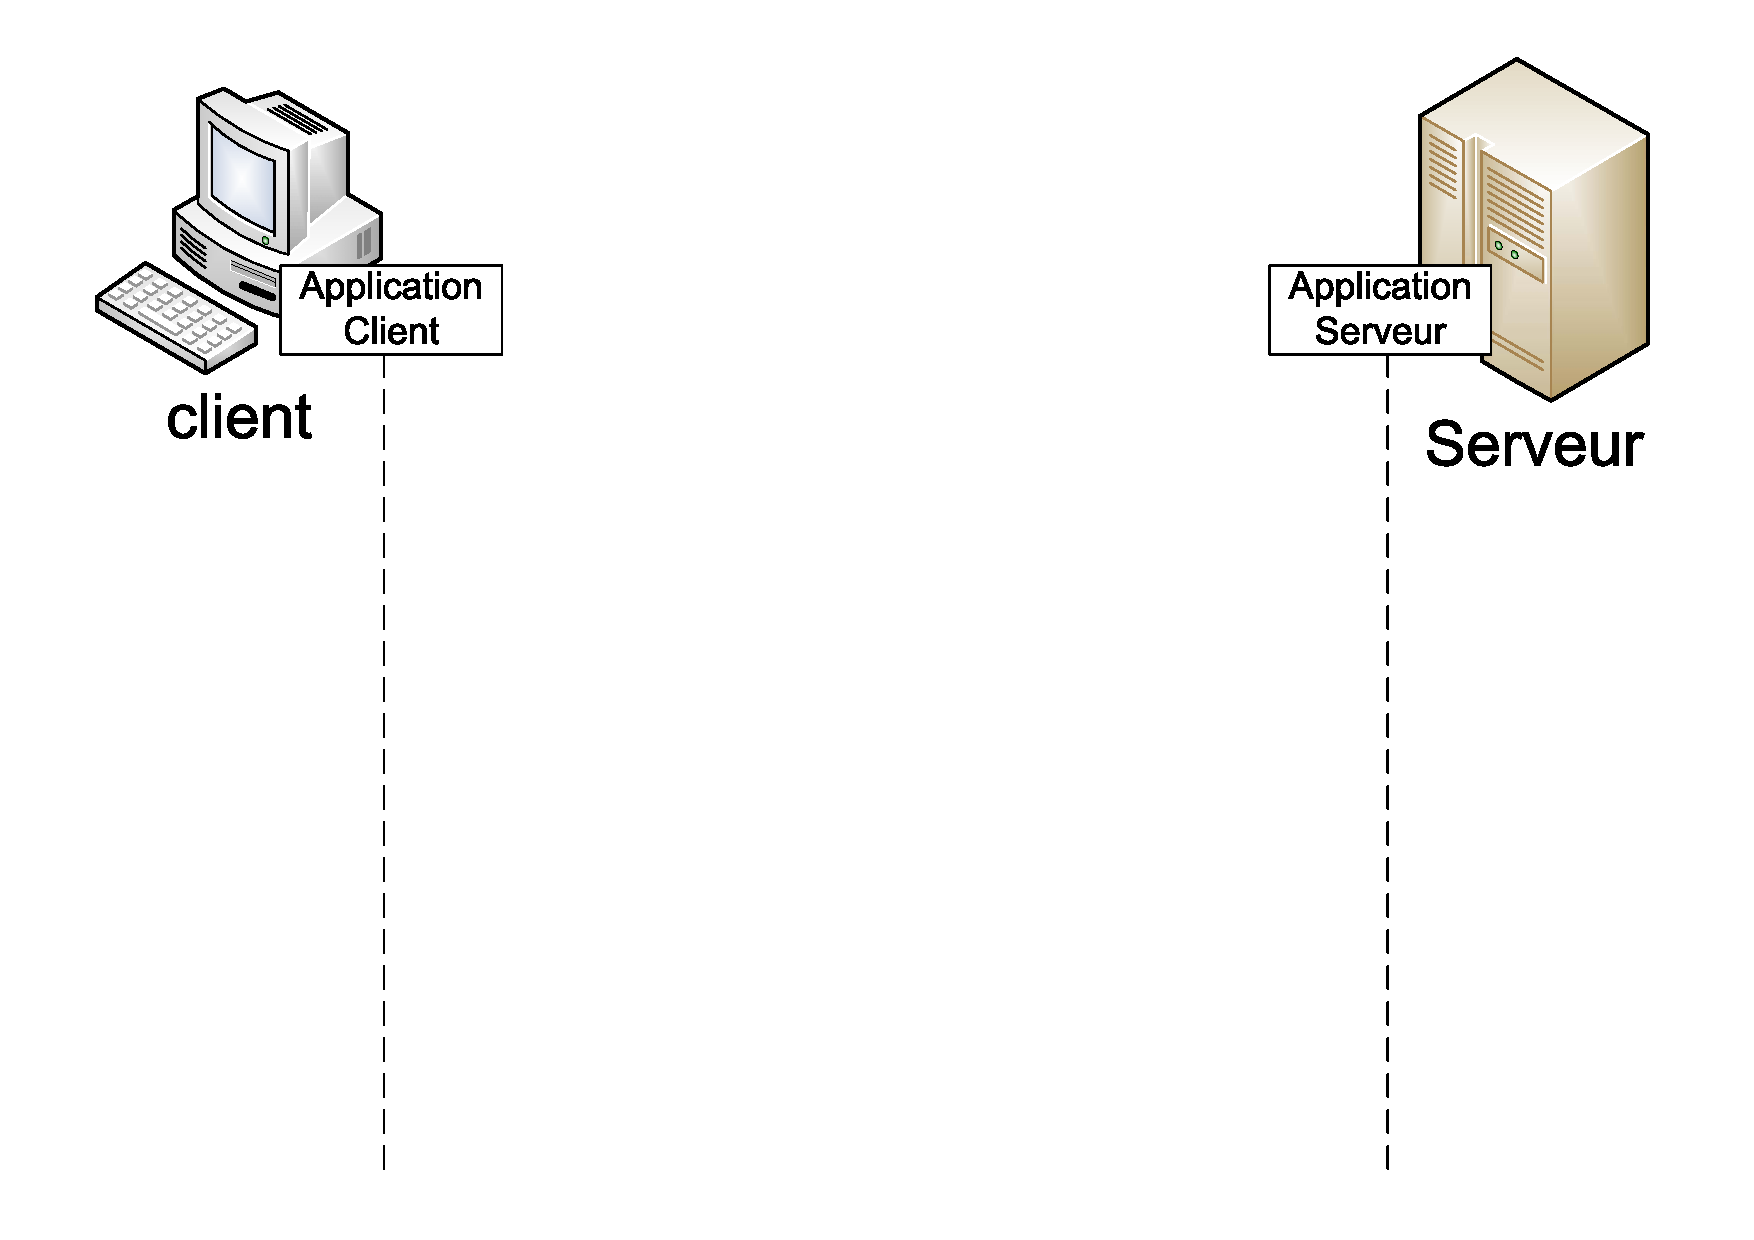
\includegraphics[width=\textwidth]{res/CSudp0.pdf}
		
\end{frame}
% ----------------------------------------------------------------------
\begin{frame}{UDP : Initialisation Socket}

	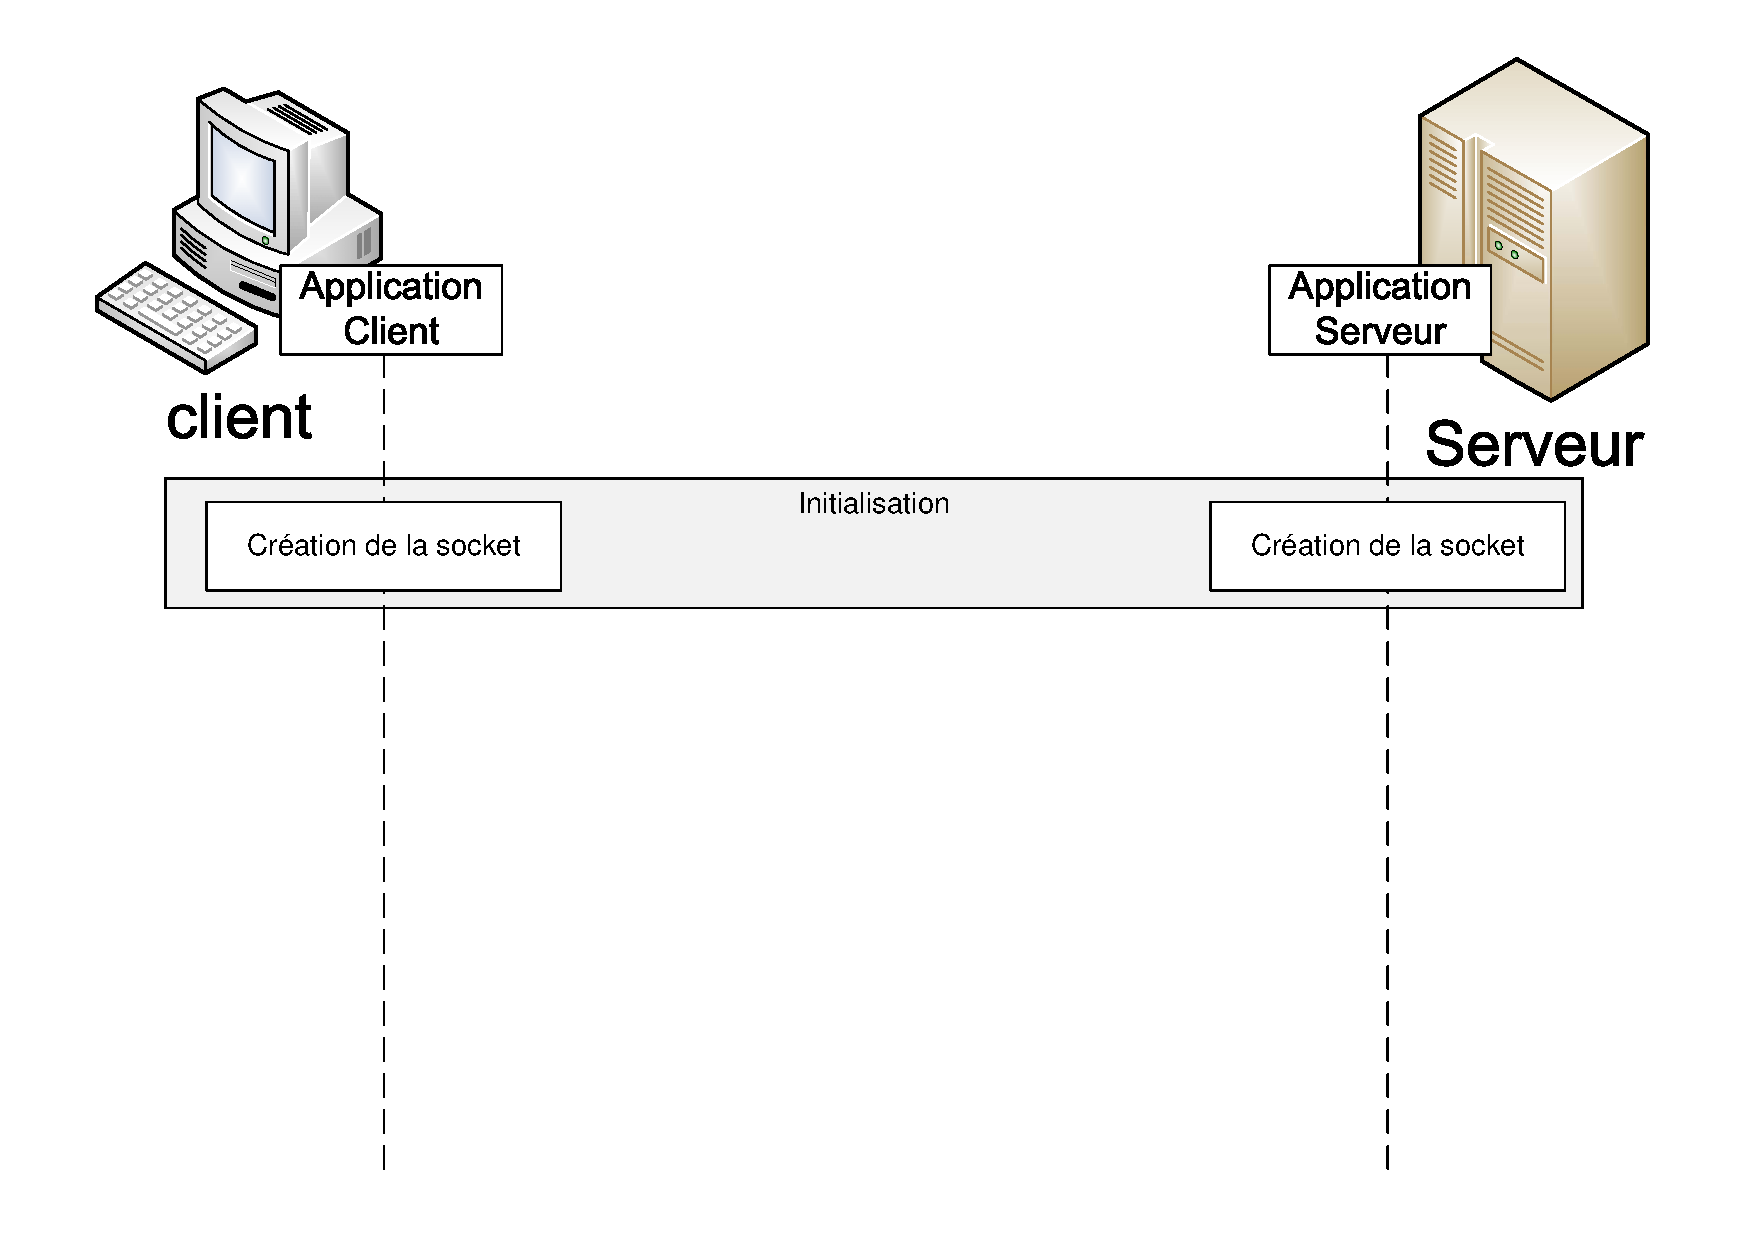
\includegraphics[width=\textwidth]{res/CSudp1.pdf}
		
\end{frame}
% ----------------------------------------------------------------------
\begin{frame}{UDP : Communications Socket}

	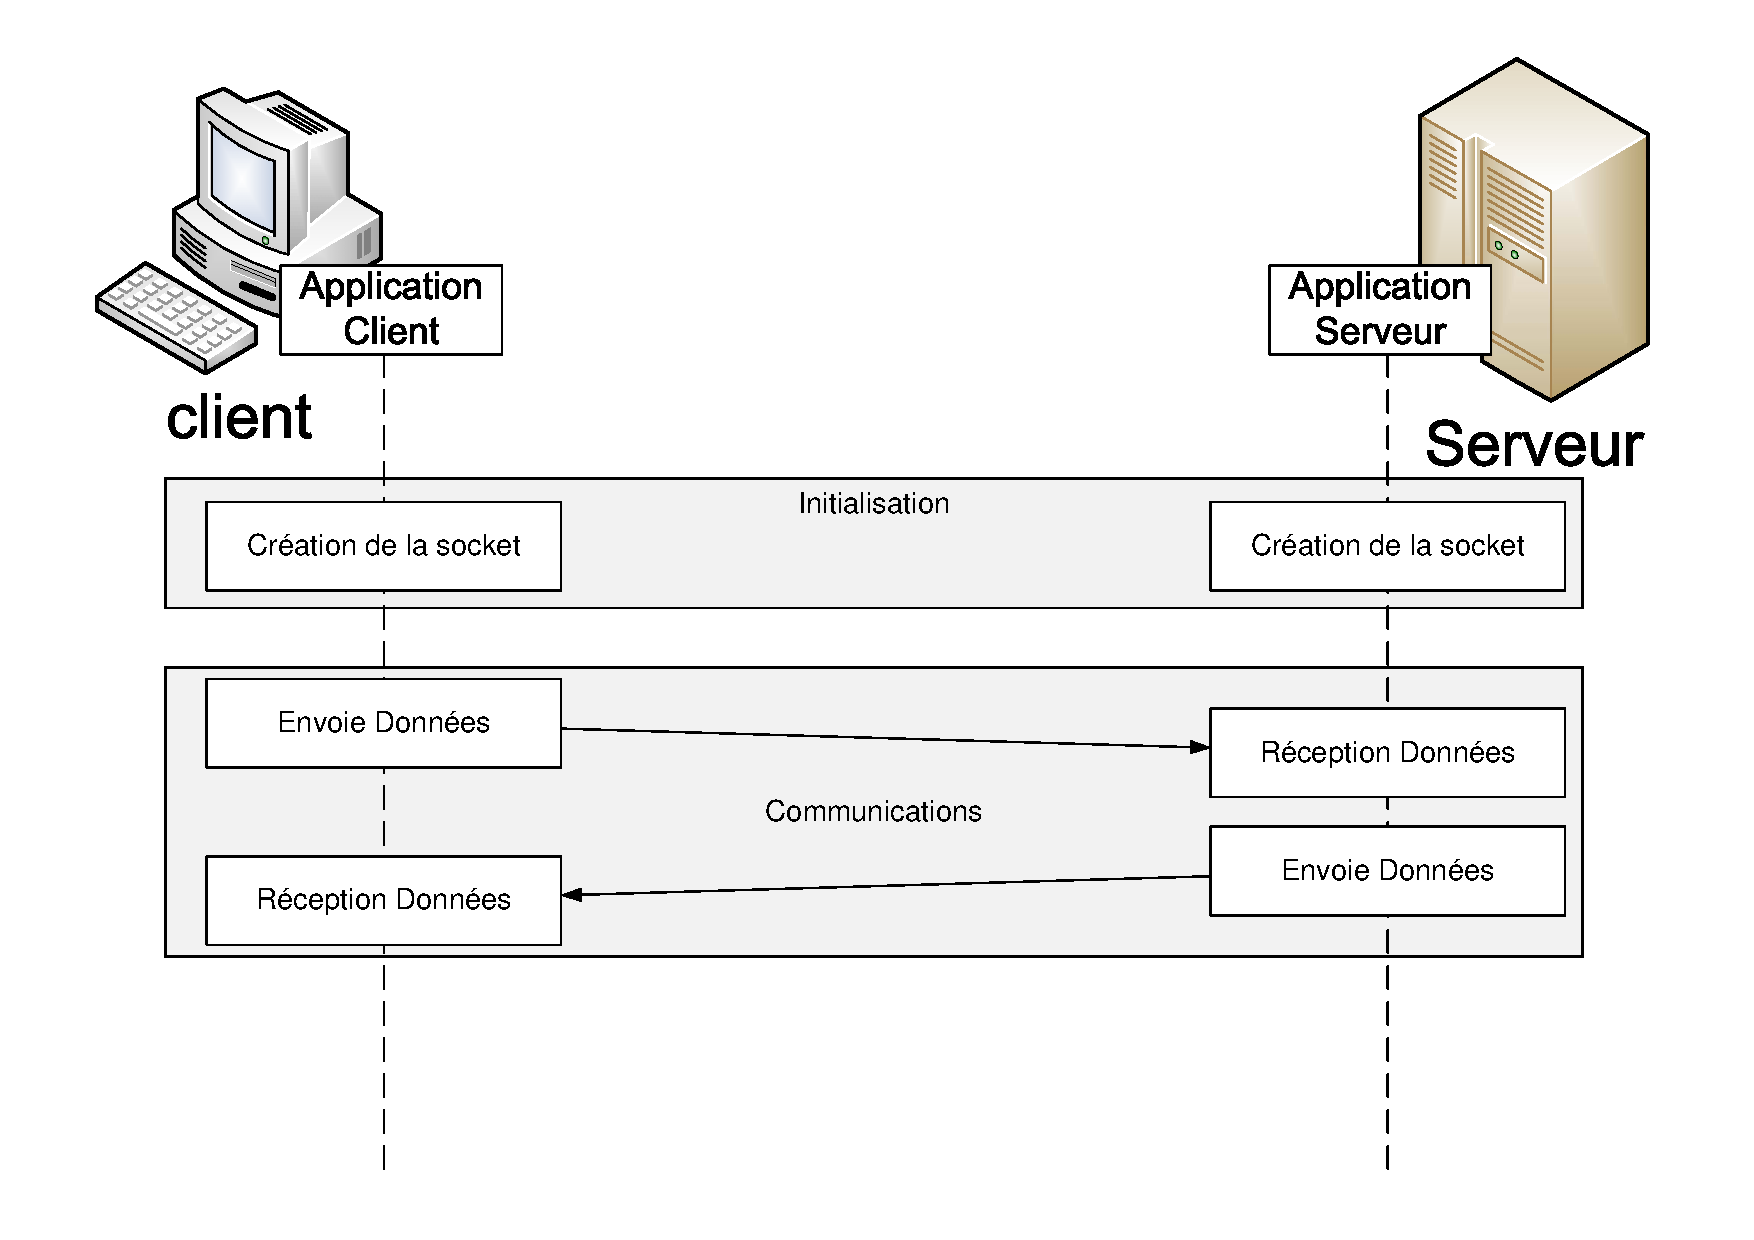
\includegraphics[width=\textwidth]{res/CSudp2.pdf}
		
\end{frame}
% ----------------------------------------------------------------------
\begin{frame}{UDP : Fermeture Socket}

	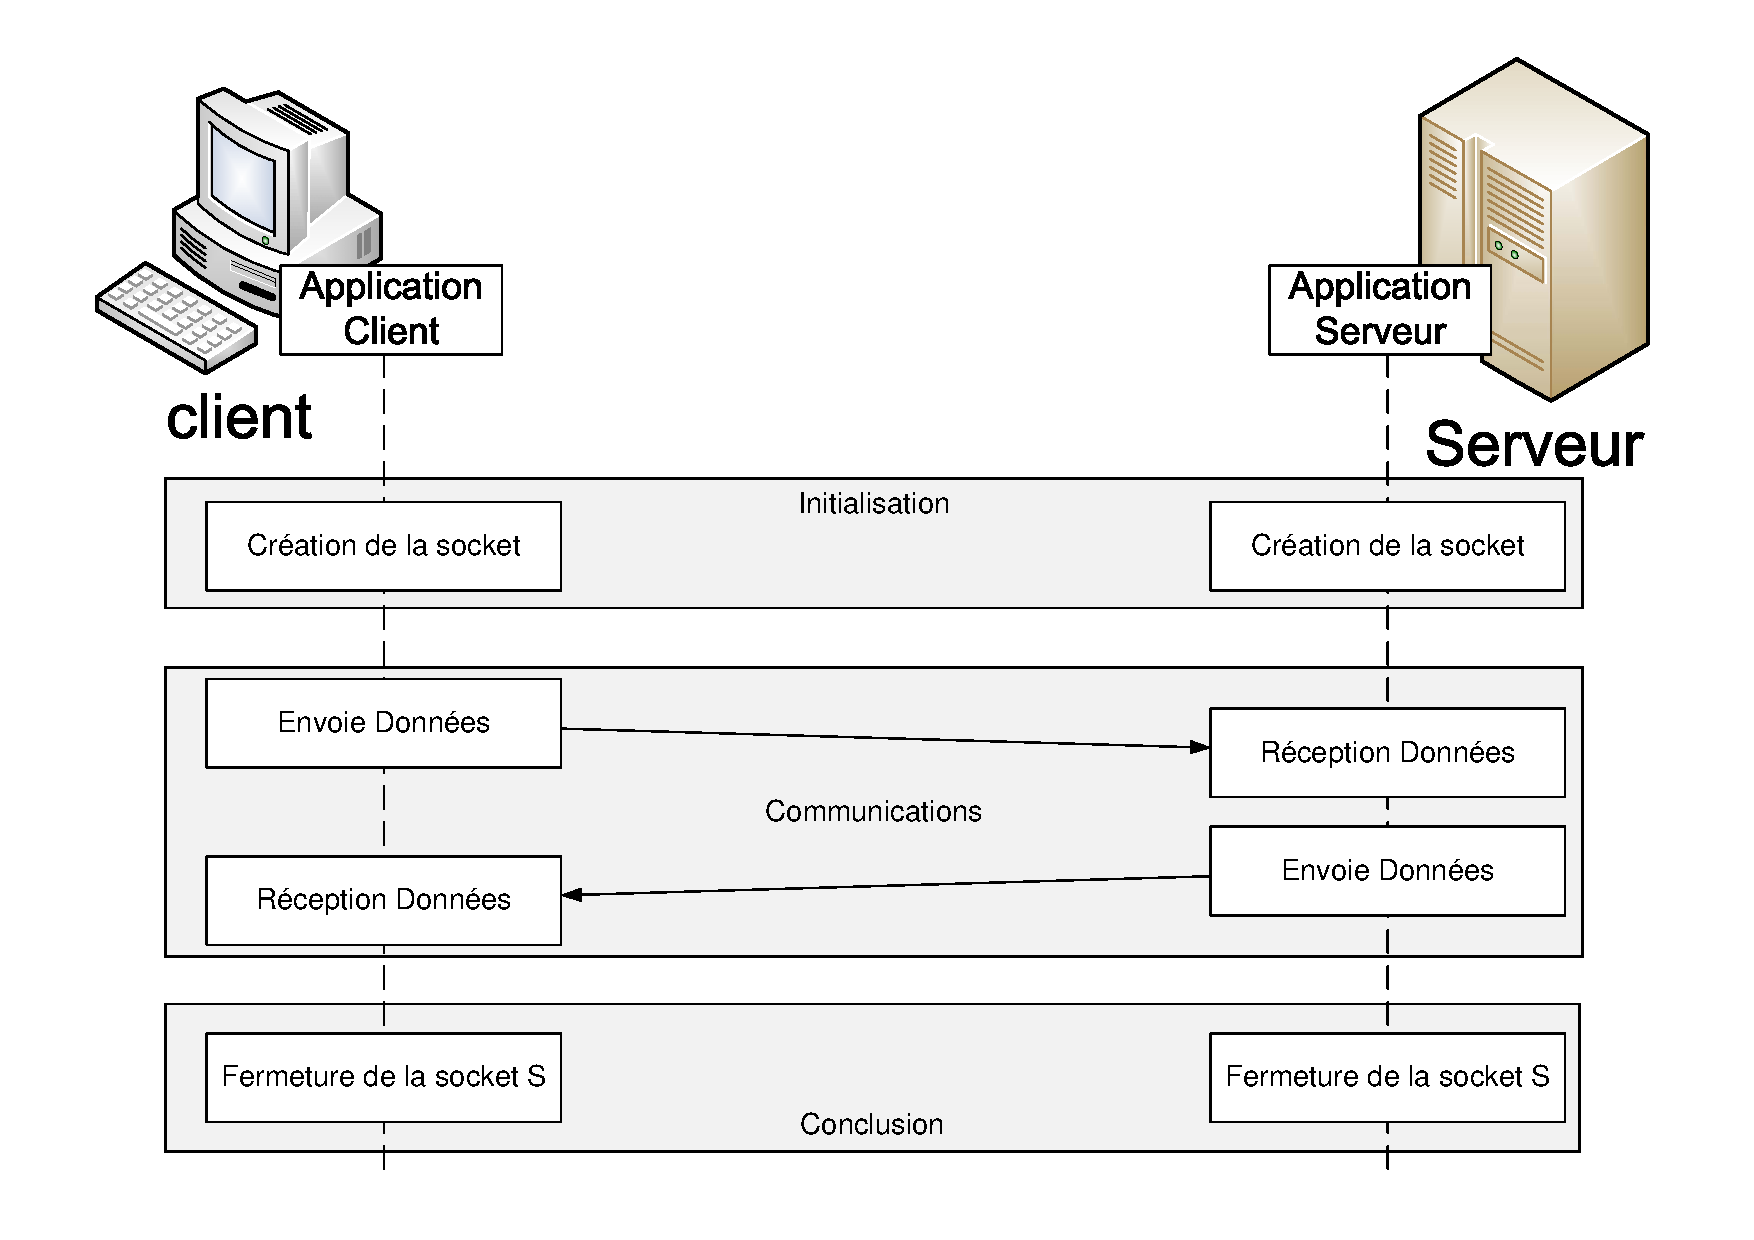
\includegraphics[width=\textwidth]{res/CSudp3.pdf}
		
\end{frame}
% ----------------------------------------------------------------------

% ----------------------------------------------------------------------
\section{Session TCP}
% ----------------------------------------------------------------------
\begin{frame}
	\begin{block}<+->{Protocole TCP}
		\begin{itemize}
		\item \textit{Transmission Control Protocol }
		\item Construit par dessus IP
		\item D�fini par la RFC793
			\begin{itemize}
			\item \url{http://tools.ietf.org/html/rfc793}
			\end{itemize}
		\item Int�gre la notion de port
		\item En mode connect�
			\begin{itemize}
			\item peu performant (beaucoup de surcharge)
			\item fiable (chaque paquet est acquitt� et checksum�)
			\end{itemize}
		\end{itemize}
	\end{block}		
\end{frame}
% ----------------------------------------------------------------------
\begin{frame}{TCP : client/serveur en mode connect�}

	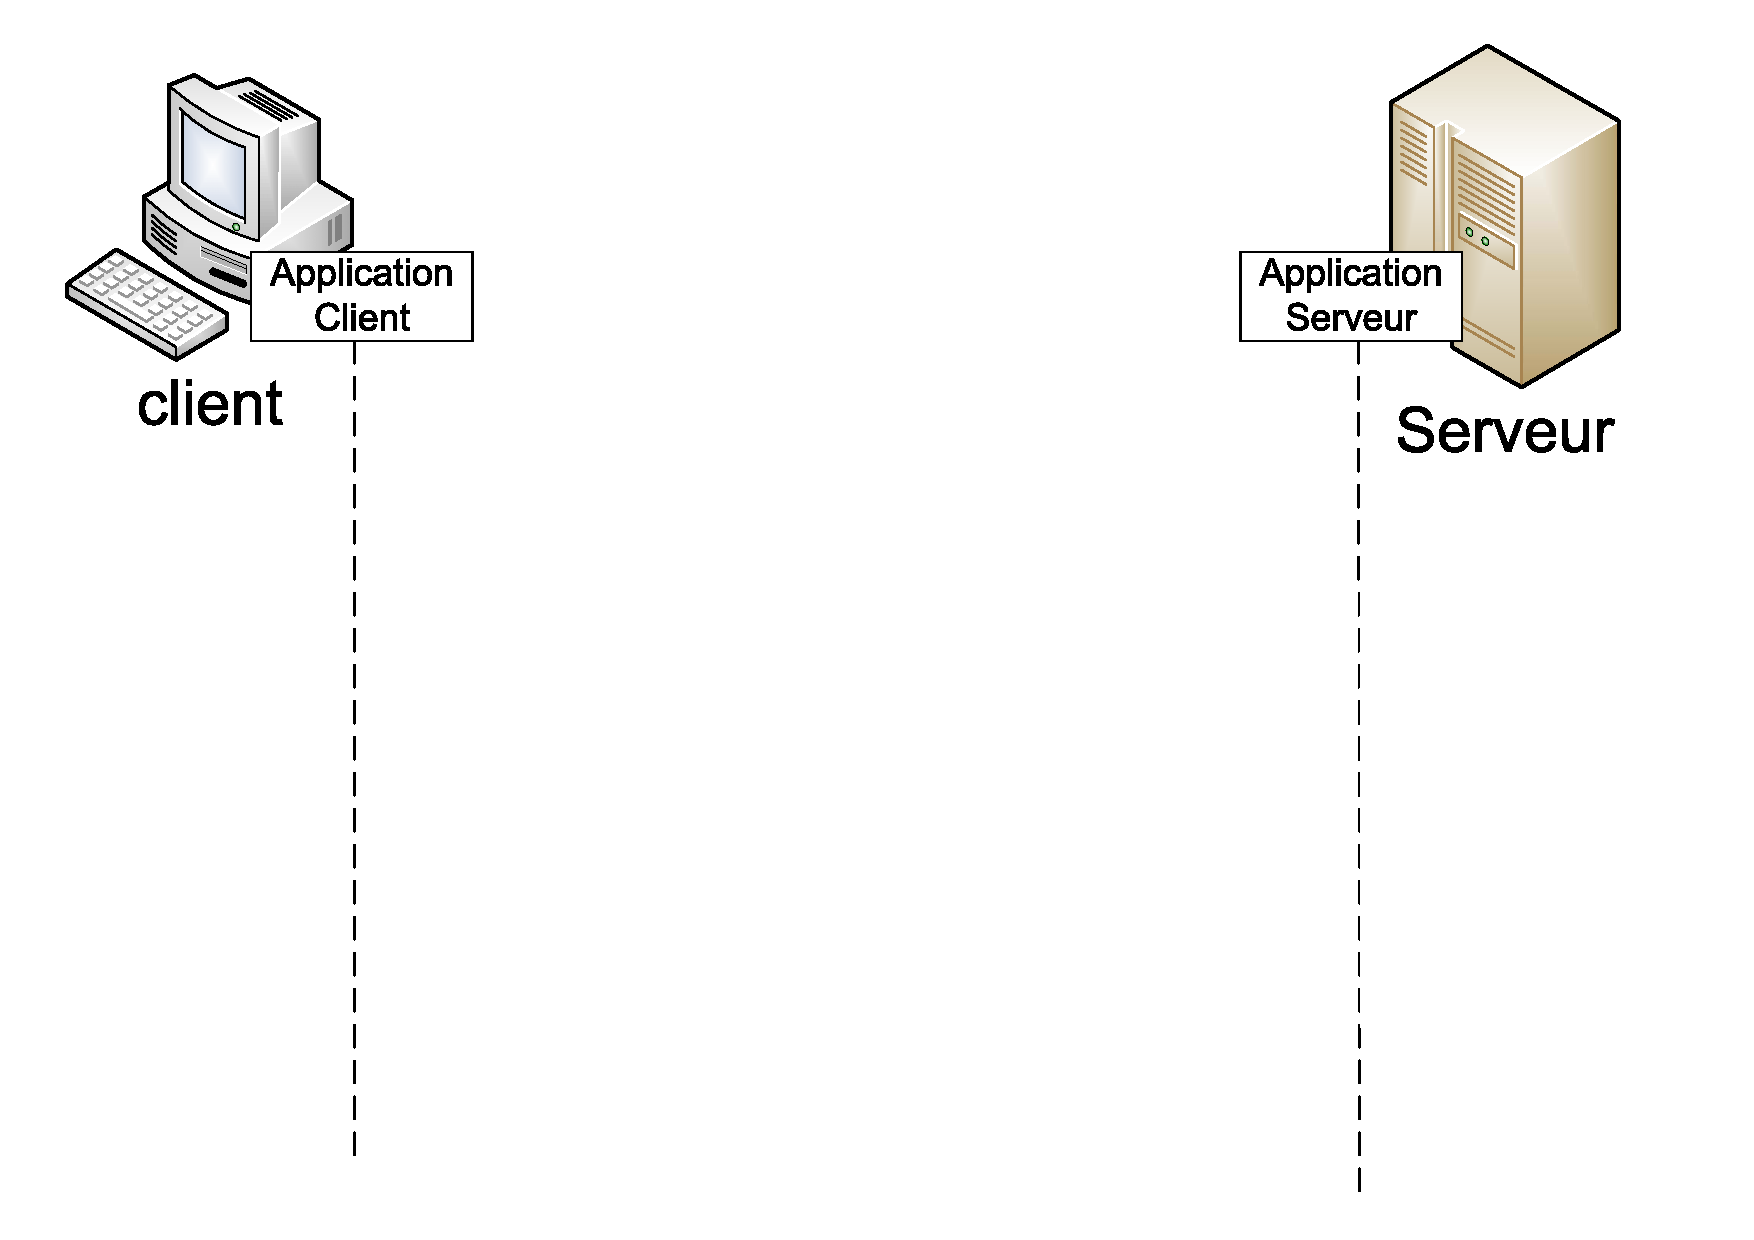
\includegraphics[width=\textwidth]{res/CStcp0.pdf}
		
\end{frame}
% ----------------------------------------------------------------------
\begin{frame}{TCP : Initialisation - Ouverture Socket - \'Ecoute}

	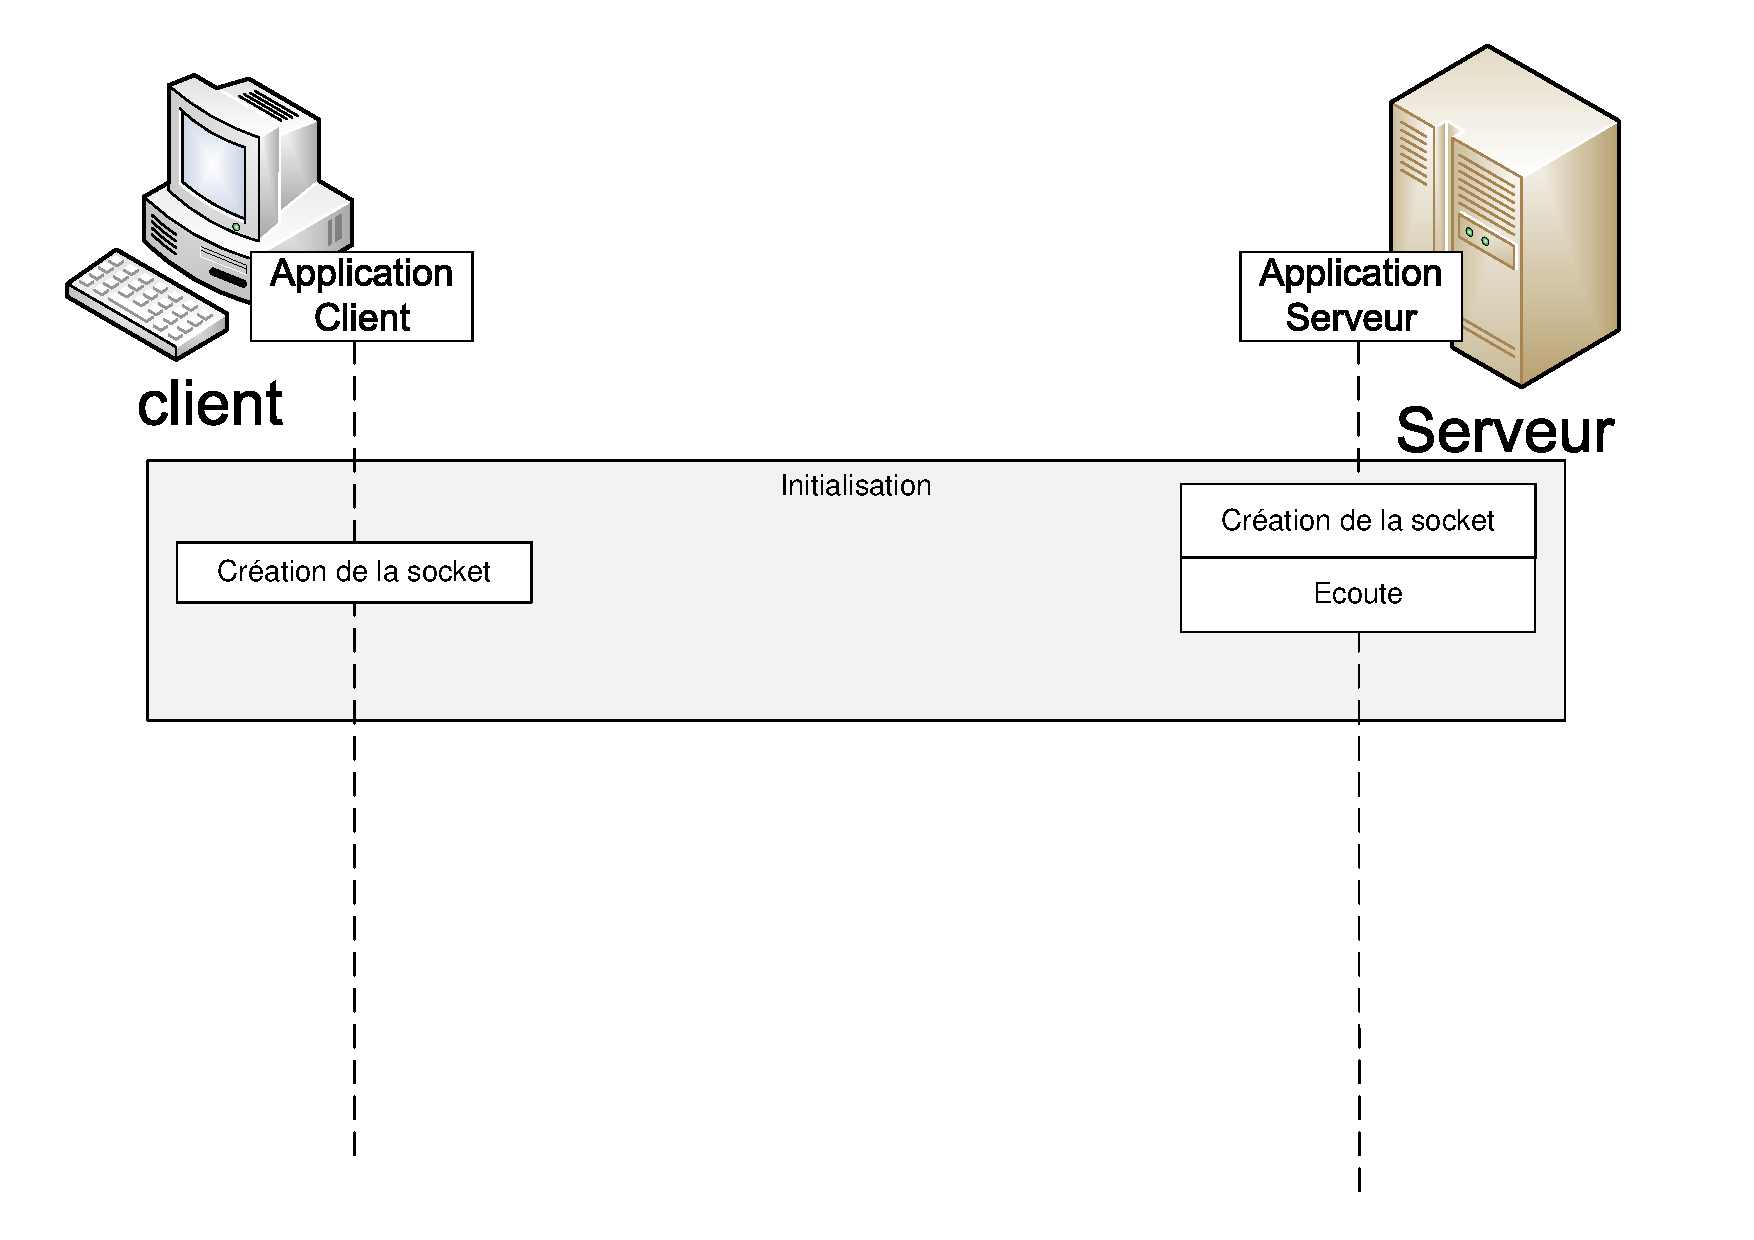
\includegraphics[width=\textwidth]{res/CStcp01.pdf}
		
\end{frame}
% ----------------------------------------------------------------------
\begin{frame}{TCP : Initialisation - Connexion}

	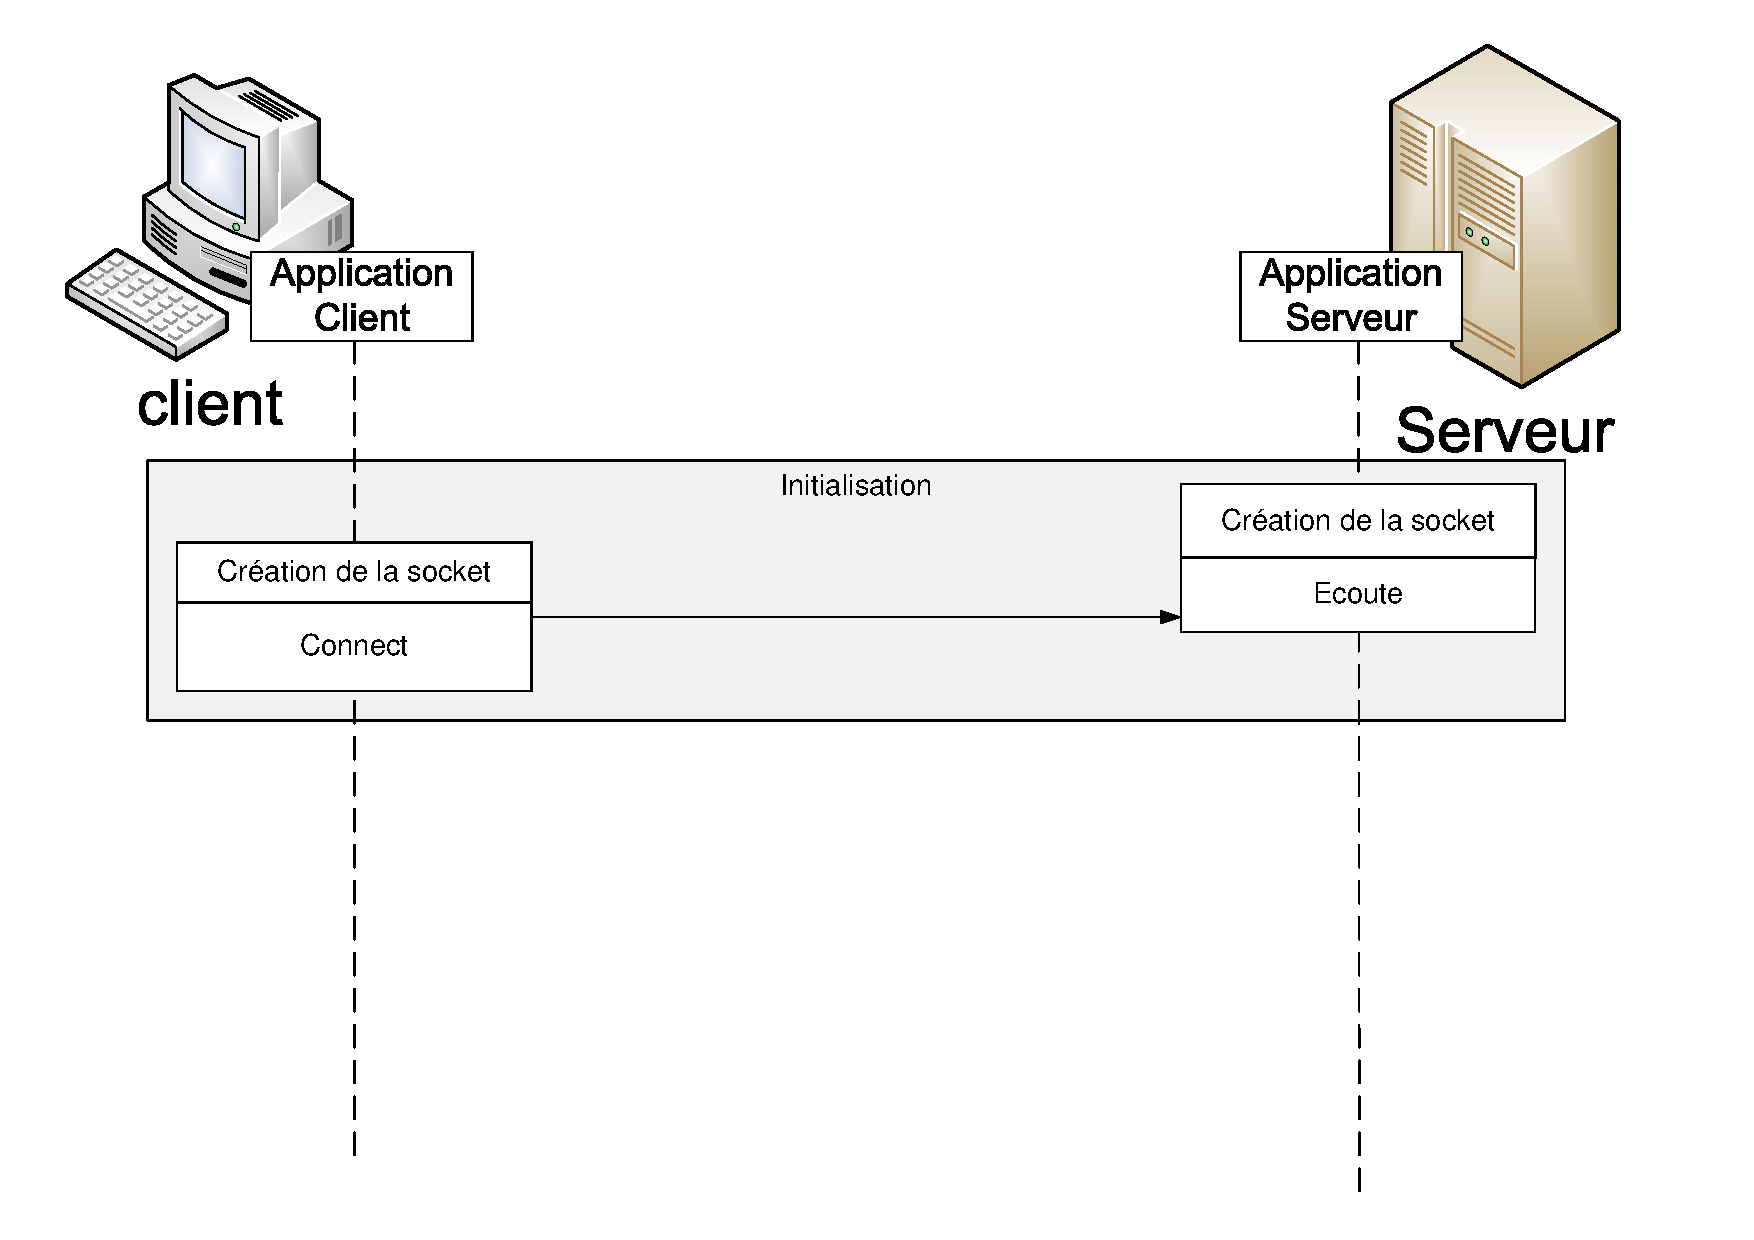
\includegraphics[width=\textwidth]{res/CStcp02.pdf}
		
\end{frame}
% ----------------------------------------------------------------------
\begin{frame}{TCP : Initialisation - Acceptation}

	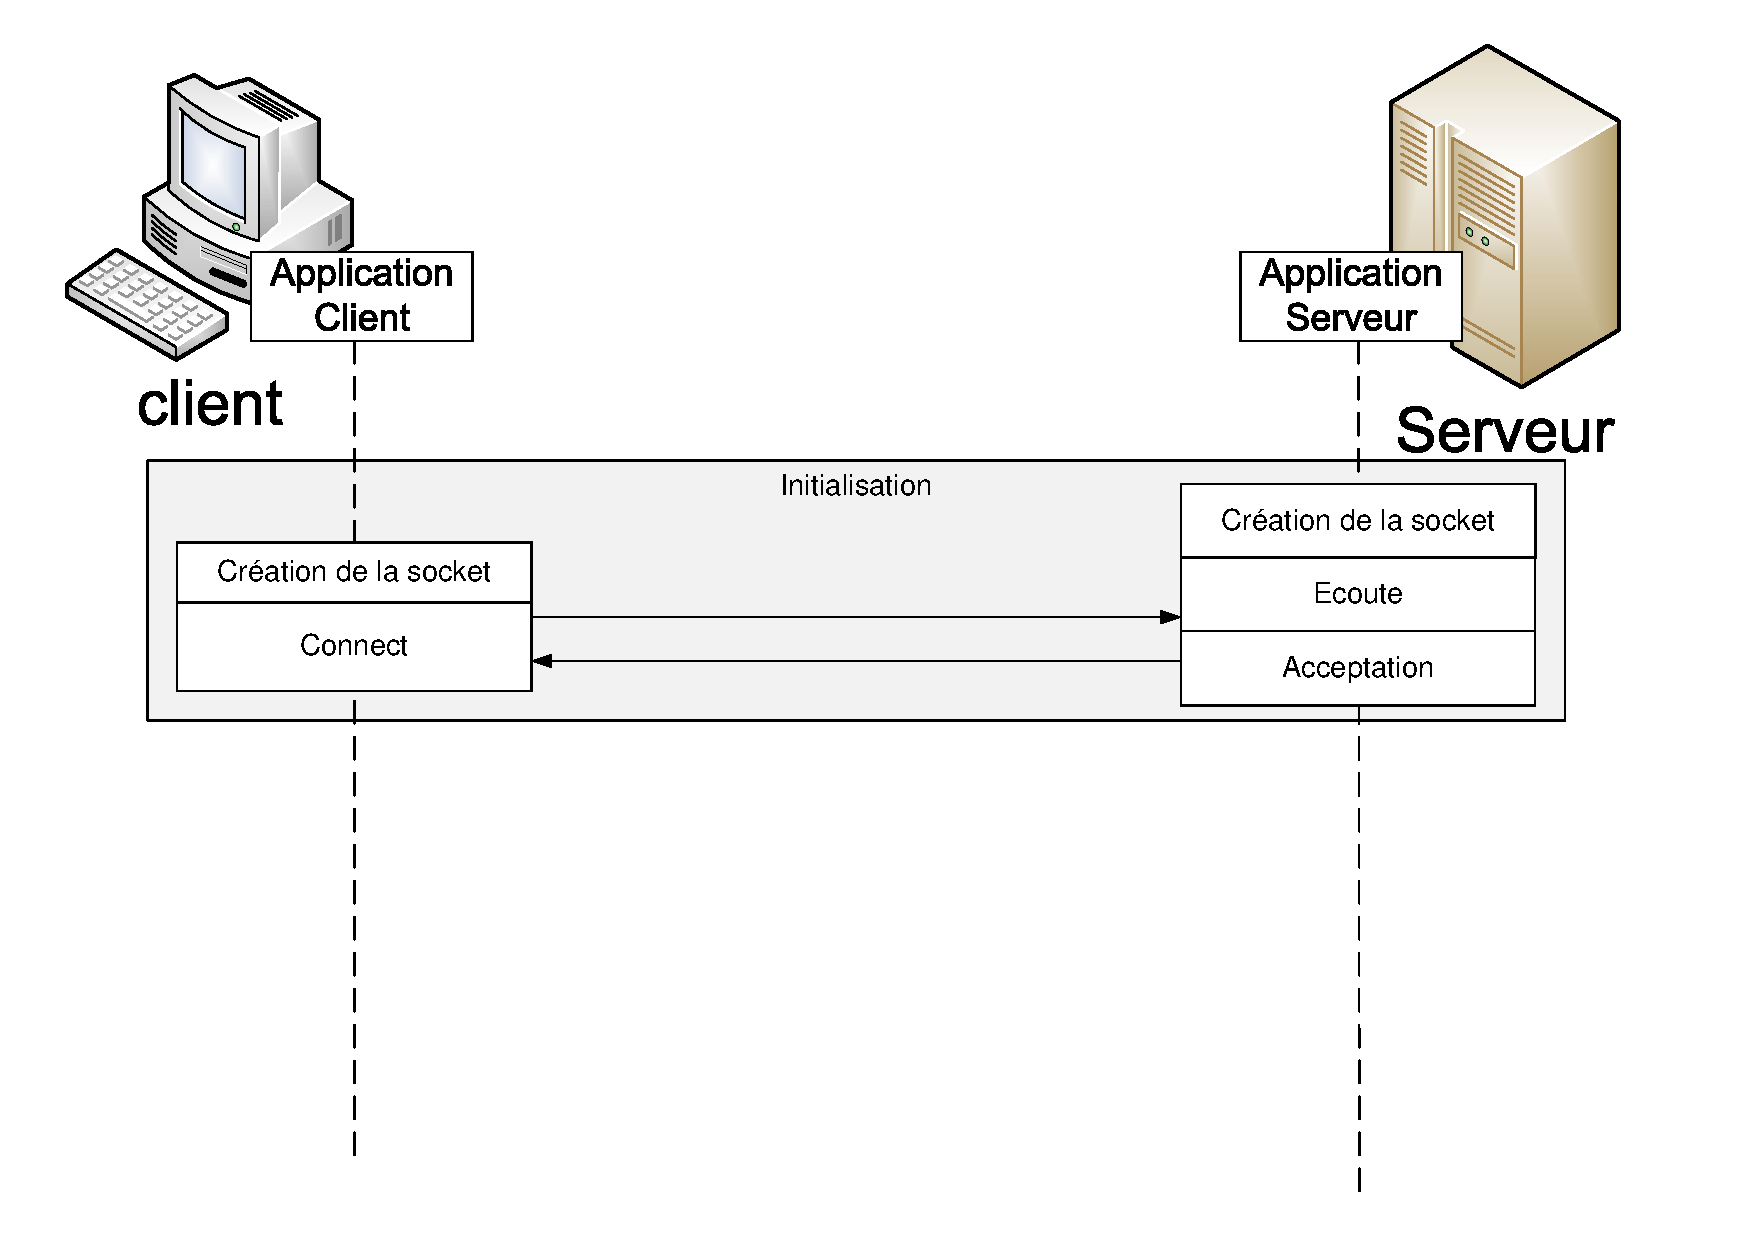
\includegraphics[width=\textwidth]{res/CStcp1.pdf}
		
\end{frame}
% ----------------------------------------------------------------------
\begin{frame}{TCP : Communication Socket}

	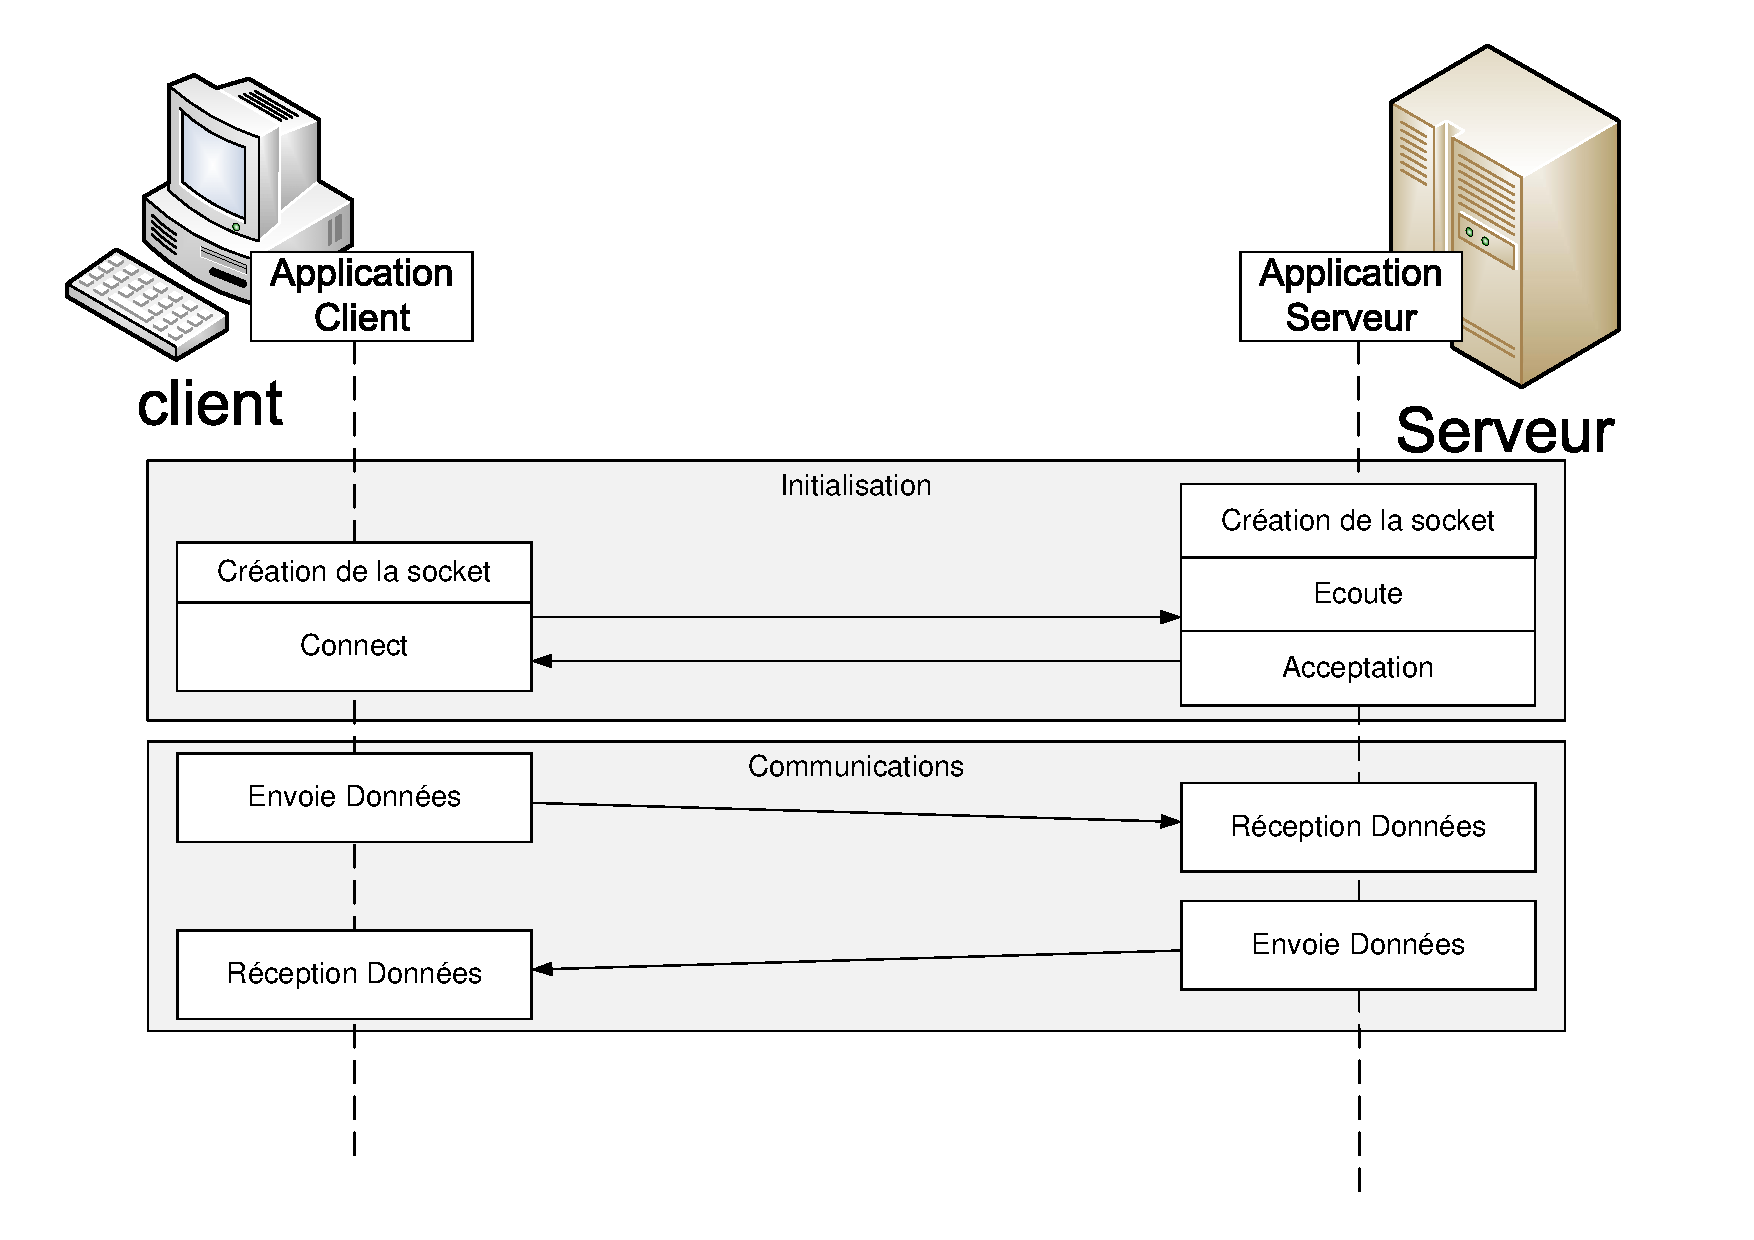
\includegraphics[width=\textwidth]{res/CStcp2.pdf}
		
\end{frame}
% ----------------------------------------------------------------------
\begin{frame}{TCP : Conclusion Socket}

	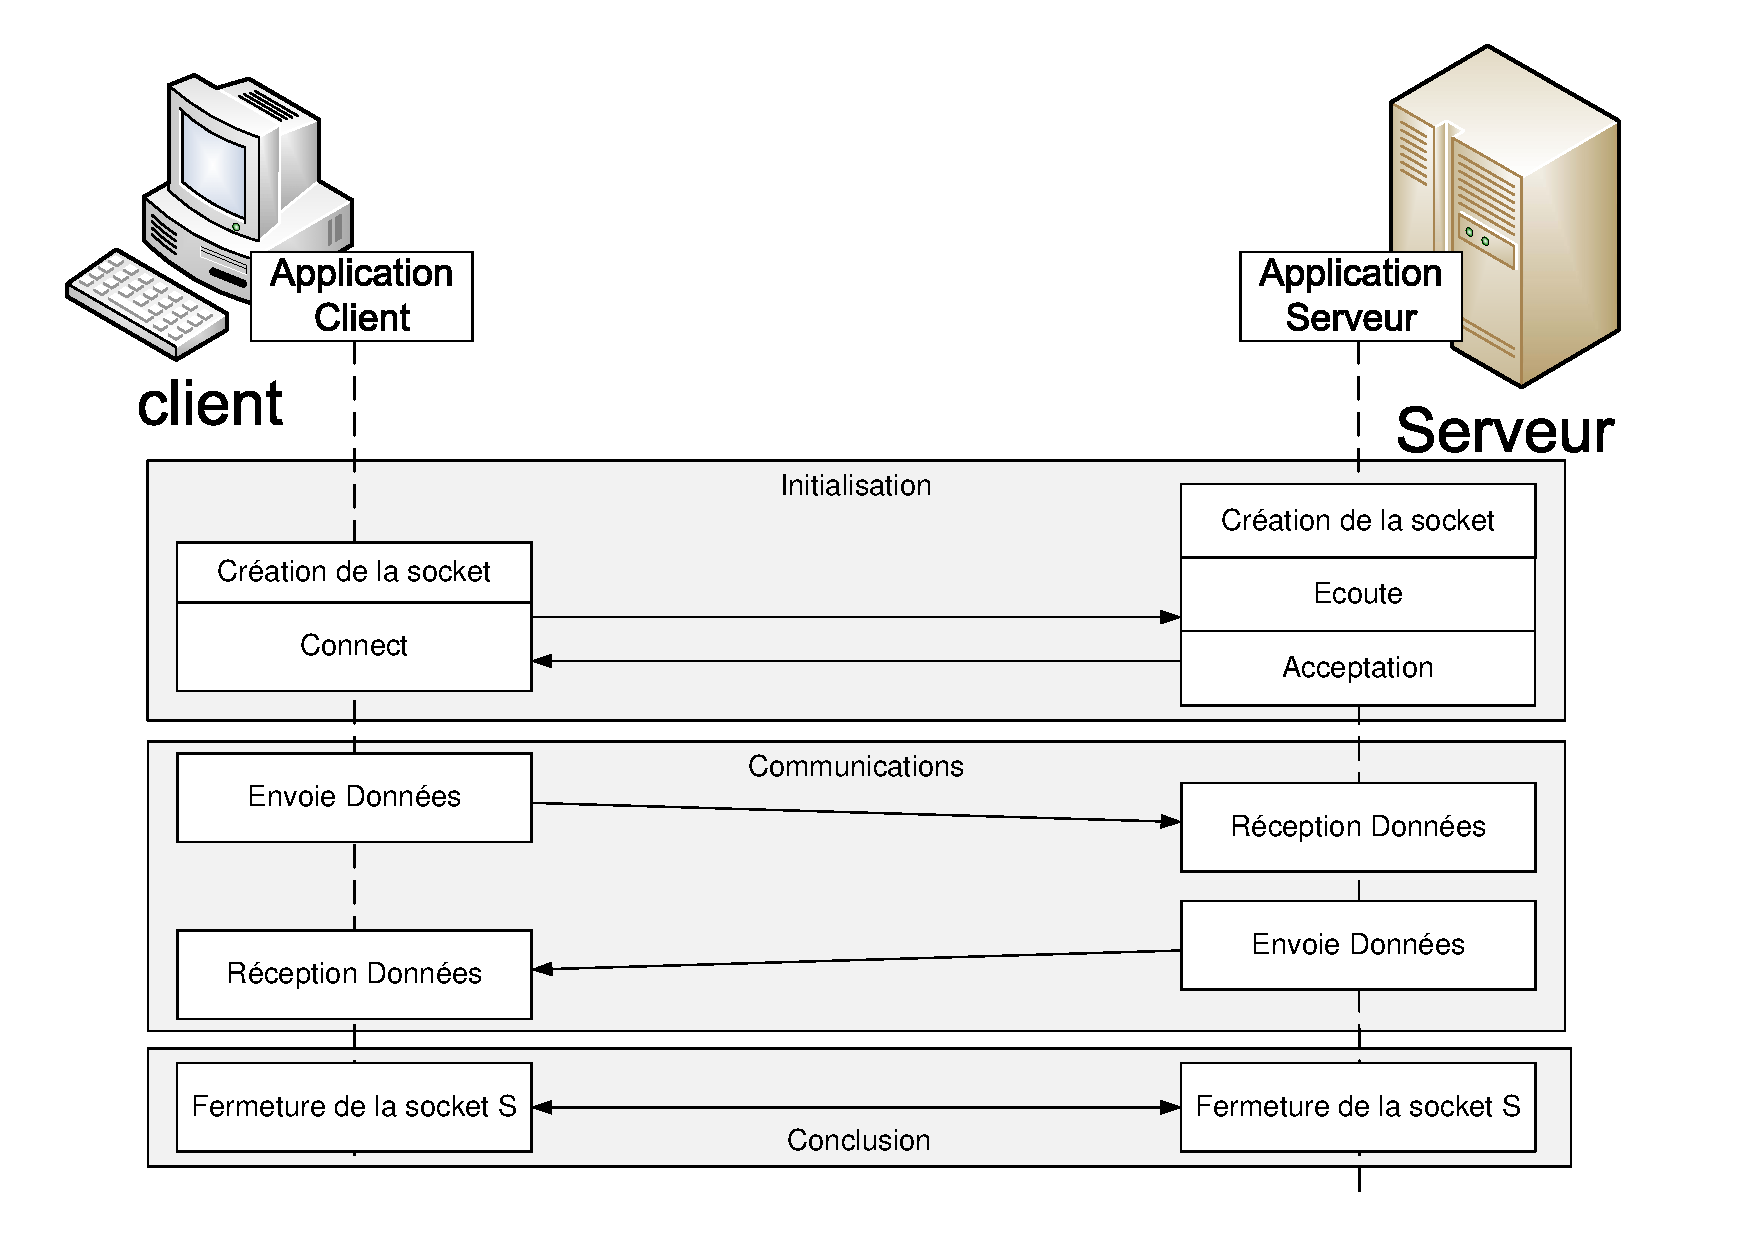
\includegraphics[width=\textwidth]{res/CStcp3.pdf}
		
\end{frame}
% ----------------------------------------------------------------------
\begin{frame}{TCP : Retour � l'\'Ecoute du prochain client}

	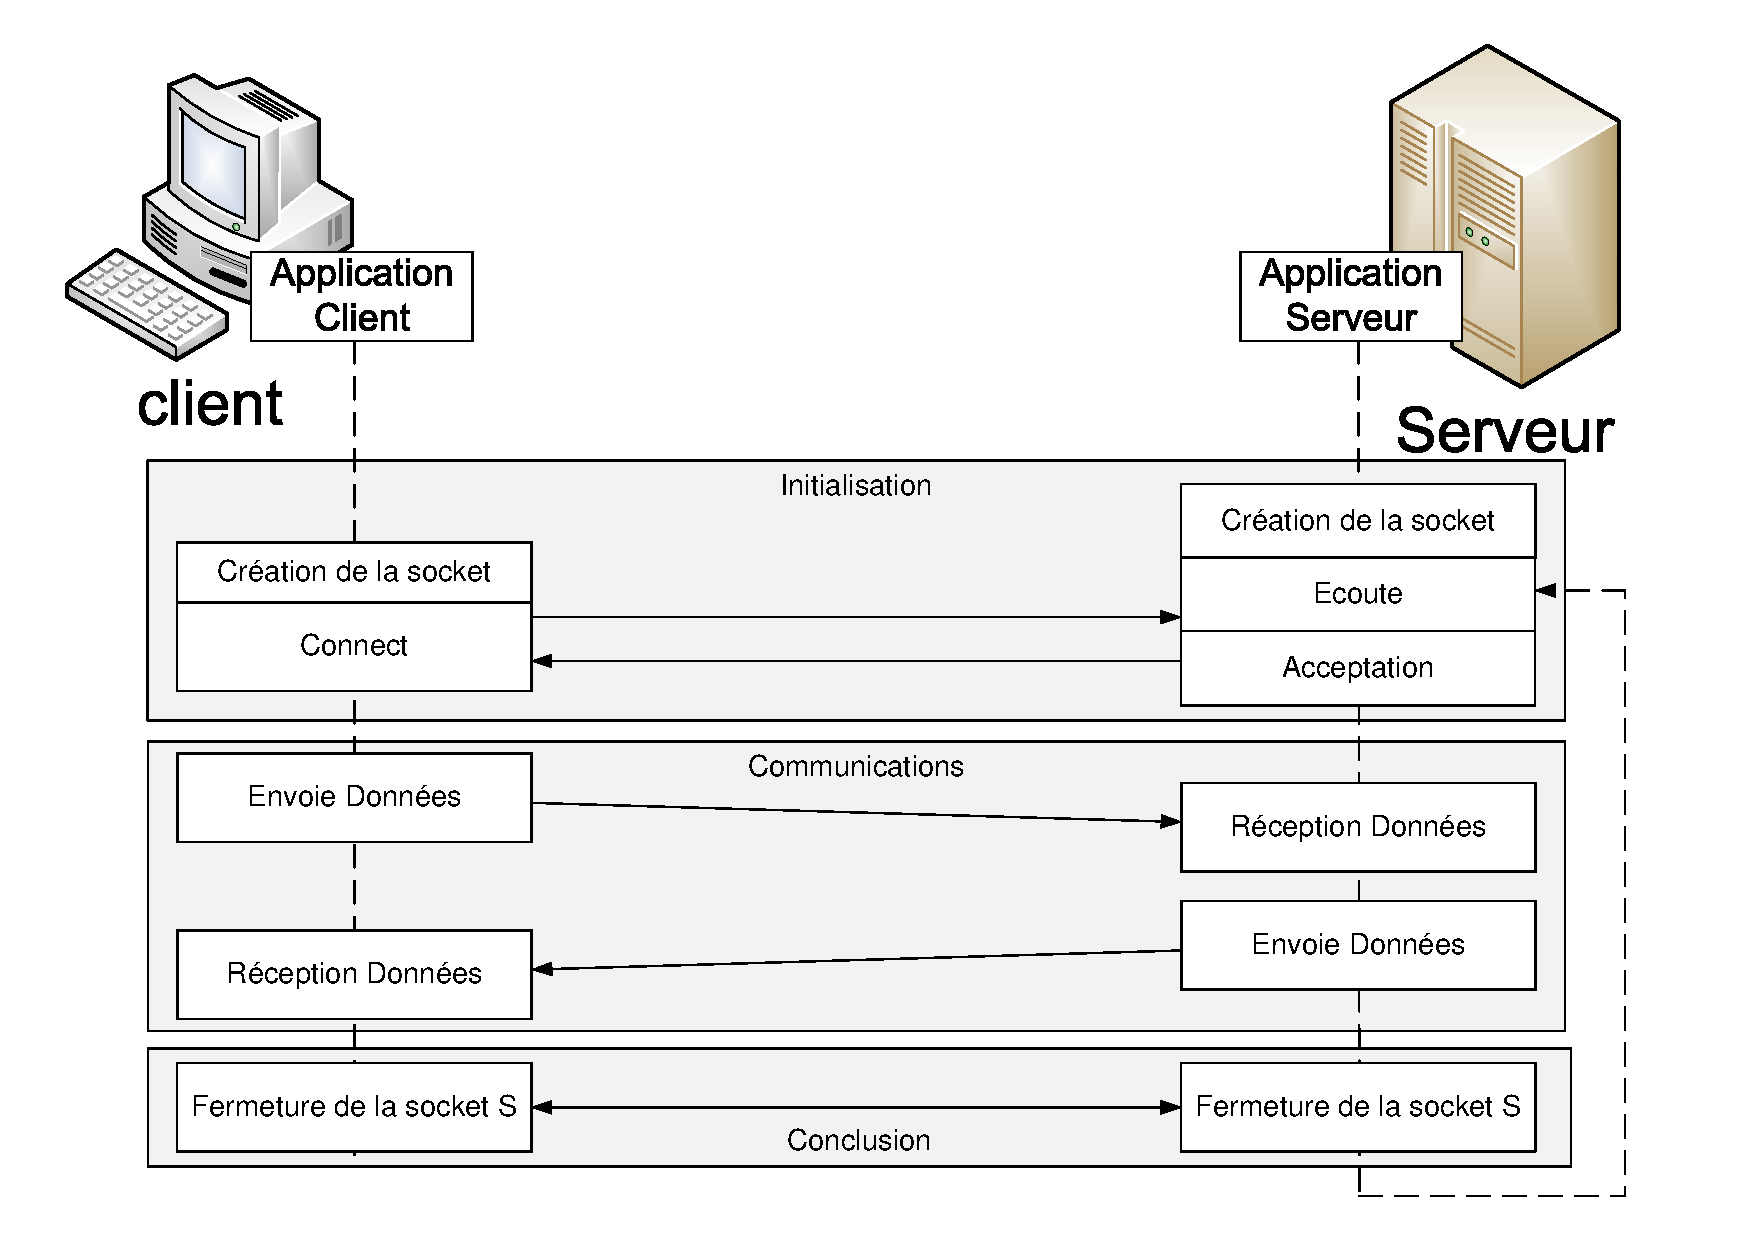
\includegraphics[width=\textwidth]{res/CStcp4.pdf}
		
\end{frame}
% ----------------------------------------------------------------------
\begin{frame}{TCP : Multi-Clients Simultan�s}

	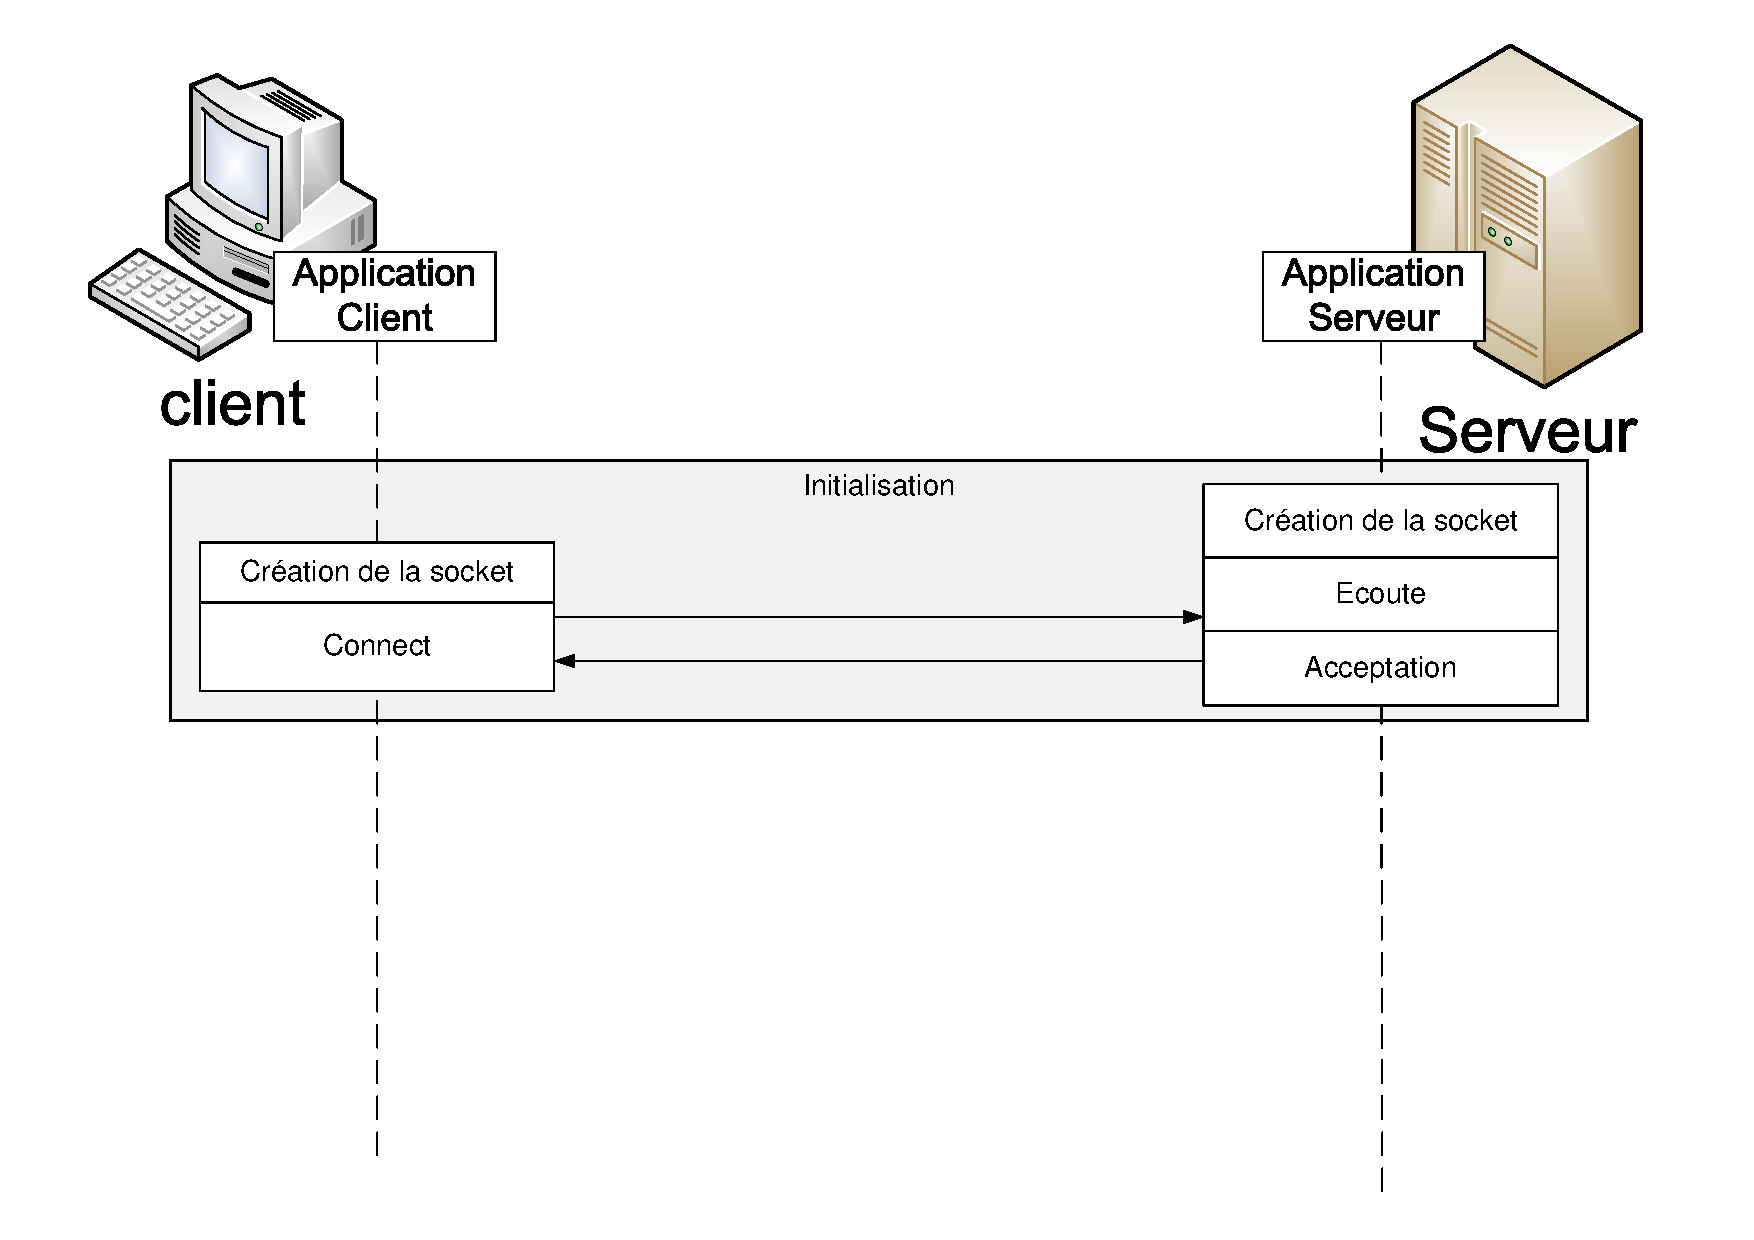
\includegraphics[width=\textwidth]{res/CStcp5.pdf}
		
\end{frame}
% ----------------------------------------------------------------------
\begin{frame}{TCP : Fork (mitose du processus)}

	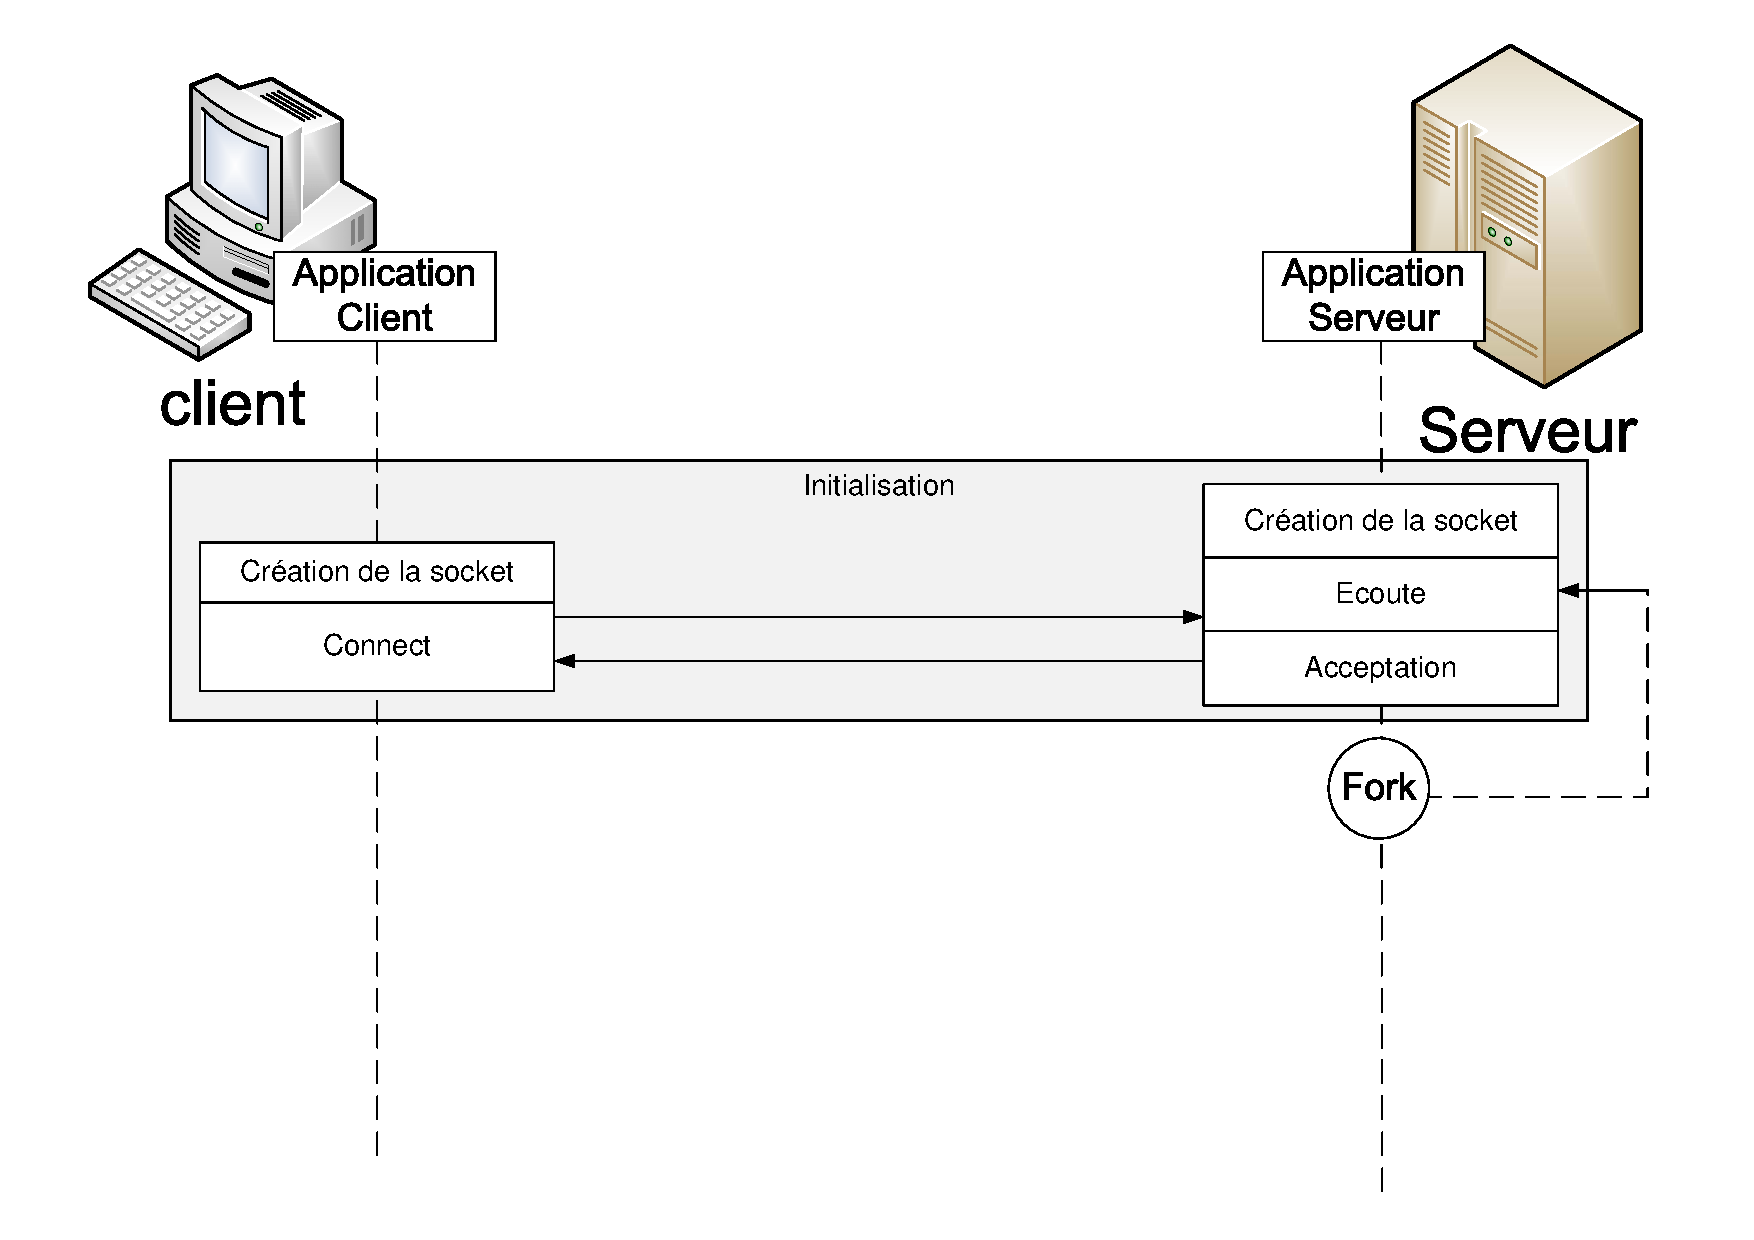
\includegraphics[width=\textwidth]{res/CStcp6.pdf}
		
\end{frame}
% ----------------------------------------------------------------------
\begin{frame}{TCP : Suite PENDANT \'Ecoute}

	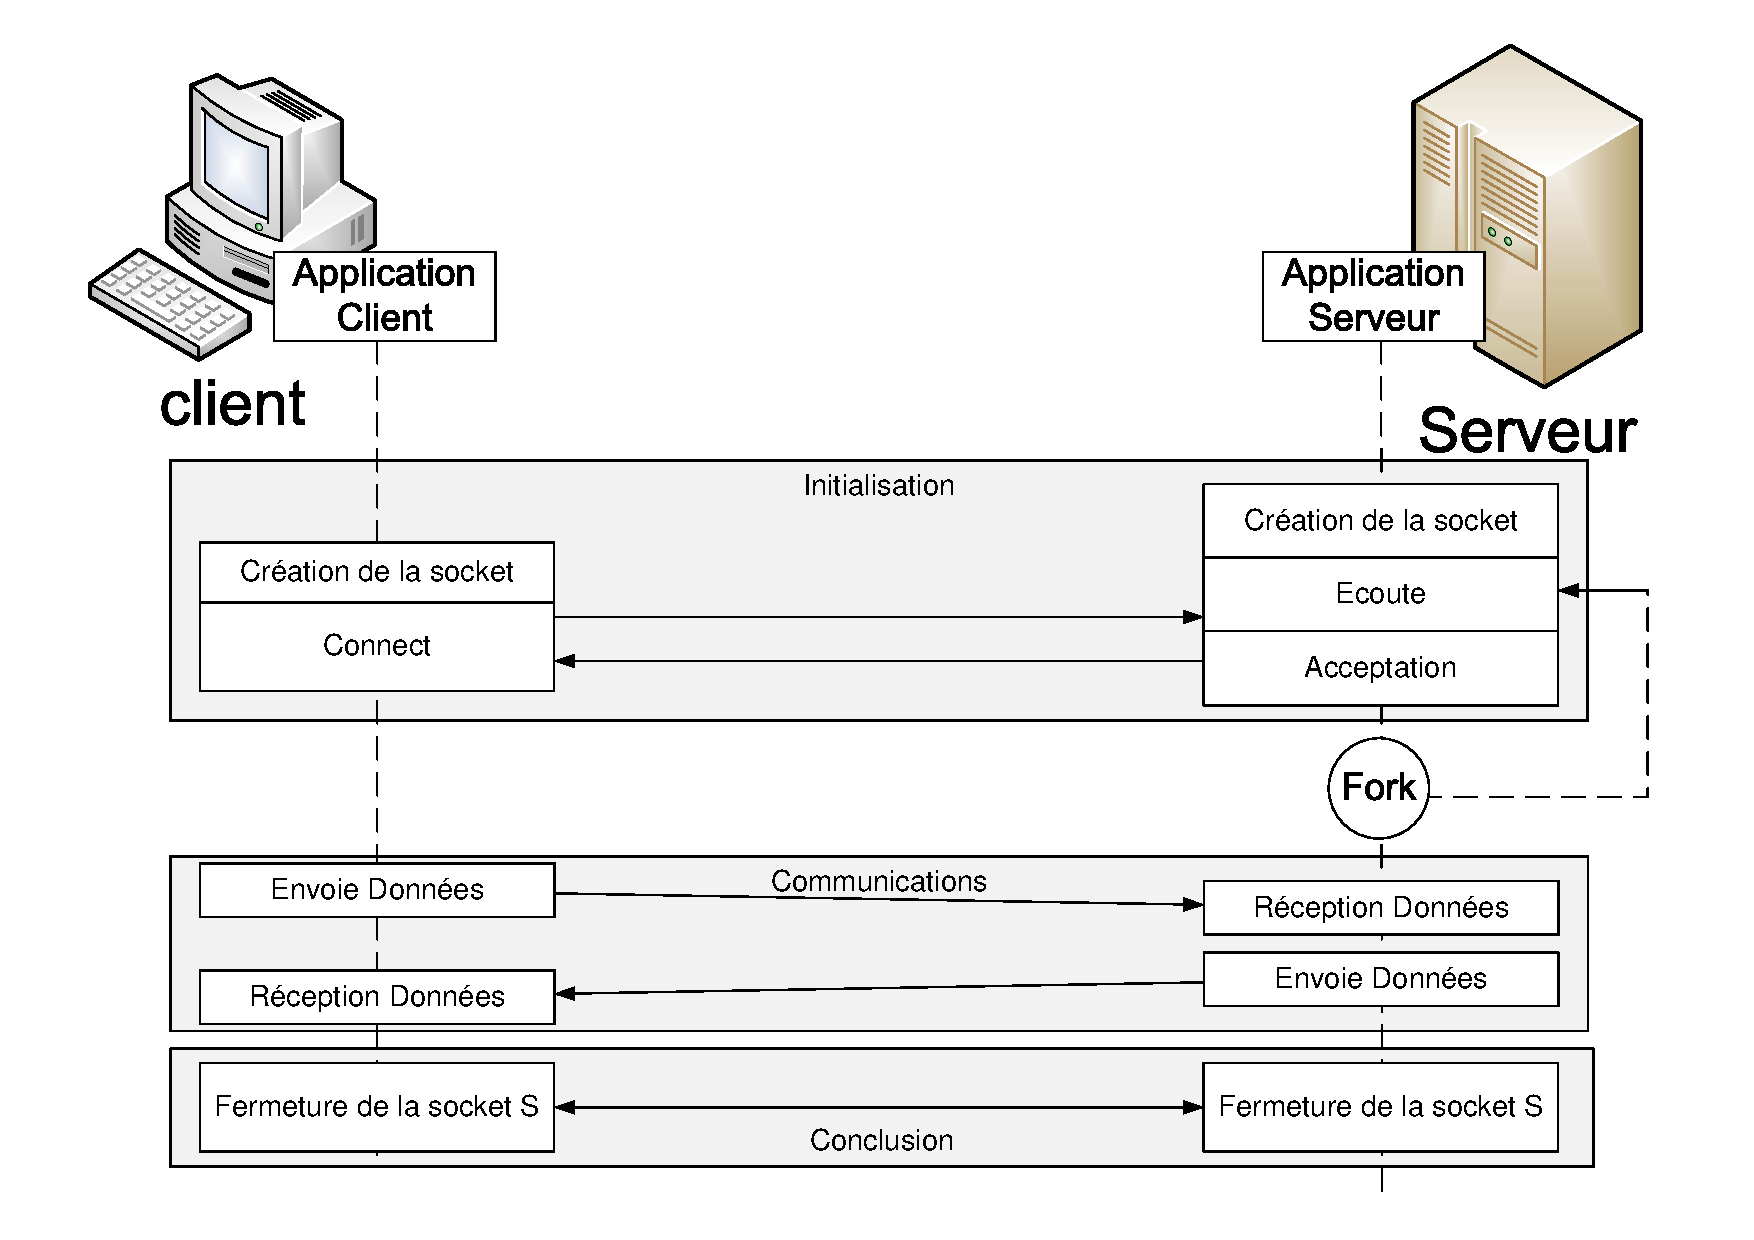
\includegraphics[width=\textwidth]{res/CStcp7.pdf}
		
\end{frame}
% ----------------------------------------------------------------------

\begin{frame}{Conclusion}
\tableofcontents
\end{frame}

\end{document}